\documentclass[a4paper]{article}

\setlength{\oddsidemargin}{-4mm}
\addtolength{\topmargin}{-1in}
\addtolength{\footskip}{+0.5in}
\addtolength{\textwidth}{+1.5in}
\addtolength{\textheight}{+1in}

\usepackage[utf8]{inputenc}
\usepackage[english]{babel}
\usepackage{listings}
\usepackage{color}
\usepackage{multirow}
\usepackage{rotating}
\usepackage{graphicx}
\usepackage{caption}
\usepackage{amsmath}
\usepackage{subfig}
\usepackage{hyperref}
\hypersetup{linktocpage}
\renewcommand{\familydefault}{cmr}

\title{Report of Click Labs \\
Network management and QoS provisioning Course}
\author{Hong-Nam Hoang, Manh-Ha Nguyen and Xuan-Thu Thi Le}
\date{\today}

\begin{document}
  \maketitle
  \tableofcontents

  \definecolor{stringcolor}{rgb}{0.20,0.50,0.20}
  \definecolor{commentcolor}{rgb}{0.40,0.40,0.40}
  \definecolor{keywordcolor}{rgb}{0.50,0.10,0.10}
  \definecolor{idcolor}{rgb}{0.10,0.10,0.50}
  \definecolor{bg}{rgb}{0.95,0.95,0.95}  
  \lstdefinestyle{C}{basicstyle=\ttfamily,
                          keywordstyle=*\color{keywordcolor}\bfseries,
                          identifierstyle=\color{idcolor},
                          commentstyle={\color{black}\it},
                          stringstyle={\color{stringcolor}\ttfamily},
                          showstringspaces=false,
                          breaklines=true,
                          numbers=left,
                          numbersep=10pt,
                          stepnumber=1,
                          numberstyle=\small,
                          frame=single,
                          }

  \lstdefinelanguage[]{Click}[]{SQL}{
    morekeywords={elementclass, Counter, InfiniteSource, RateSource, Print, Paint, PaintSwitch, Script}}

  \section{Introduction - ClickLabs package}
    \subsection{File organization}
      \begin{description}
      	\item[elements/] This directory contains all the additional Click elements using in the lab. At this time, it includes:
      	\begin{itemize}
      		\item \texttt{randinfinitesource.\{hh,cc\}}: Similar \texttt{InfiniteSource} but random byte value in payload.
      		\item \texttt{randomqueue.\{hh,cc\}}: Random Queue.
      		\item \texttt{setvirtualclock.\{hh,cc\}}: Set Virtual Clock. It is used for GCRA and Virtual clock scheduler.
      		\item \texttt{wrrsched.\{hh,cc\}}: Weighted Round Robin Scheduling.
      		\item \texttt{wdrr.\{hh,cc\}}: Weighted Deficit Round Robin Scheduling.
      	\end{itemize}
      	\item[plot-template/] This directory contains templates used for plotting data by \texttt{gnuplot}. These files are used by \texttt{draw-graph.sh}
      	\item[bin/update-elements.sh] Run this file to update the new elements implemented in directory elements (above). For more information, type: \\
      	\texttt{./update-elements.sh -h}
      	\item[bin/visual-clicky.sh]Shell script to visualize click experiment using \texttt{clicky}. For more information, type: \\ 
      	\texttt{./visual-clicky.sh -h}
      	\item[bin/init.sh]Initialize Click environment for lab. Just run \texttt{init.sh} in the first time you get this source or Click source directory changed.
      	\item[bin/eclick-compile.sh] Extend the Click file. A Click file can include another one to reuse some compound elements (similar include in C, or import in Java). File \texttt{eclick-compile.sh} is used to translate (or flatten) these extended-Click file to a normal Click file.
      	\item[bin/convert-click-dump.sh]This script used to transform dump files from Click (binary files) into text files. Note: this is one-way transformation, the binary files cannot be recovered from the text files.
      	\item[bin/draw-graph.sh] This script is used to draw graphs from data extracted in Click dump files. Just provide the dump files, this script will generate a graph for you. Note: No need to use \texttt{convert-click-dump.sh} before using \texttt{draw-graph.sh}.
      	\item[bin/draw-graph-framerelay.sh] Based on draw-graph.sh, this script helps to show the characteristics of verifying a conformance flow (which is deal with CIR, CBS, EBS).
      	\item[clicky.ccss] File supporting Clicky Cascading Style Sheets. It controls the appearance of a clicky diagram with style sheets written in a CSS-like language.      	
      	\item[1-test-config/] This folder contains Click configurations for the first part of Click Lab: \texttt{Counter\_test}, \texttt{RandomQueue}, \texttt{RandInfiniteSource}, \texttt{Random\_IP\_generator}.
      	\item[2-tcp-udp-generation/] This folder contains Click configurations for the part of TCP/UDP generator.
      	\item[3-shaper-policer/] This folder contains Click configurations for the part of Shaper and Policer: uncontrolled flows, Leaky bucket, Token bucket, negotiation with \{CBS, EBS, CIR\}, GCRA.
      	\item[4-scheduler/] This folder contains Click configurations for the part of Scheduler: FIFO, RR, DRR, WRR, WDRR, Virtual clock.
      	\item[5-congestion/] Click configurations for controlling congestion. At this time, there is only one Click configuration of WRED (Weighted-RED for two flows).
      \end{description}
    
    \subsection{Some introductions before surfing Click configurations}
      \begin{enumerate}
      	\item 
      	  First of all, initialize the Click environment for these stuffs. Run file \texttt{init.sh}: \\
      	    \texttt{chmod +x init.sh\\
      	    ./init.sh}\\
      	  Normally, this process takes long time for the first finding Click source path. To save time, you can create file \texttt{\~/.clickrc} with the content similar to this:\\
            \texttt{export CLICK\_SRC=/home/iizke/click/click-1.8.0}
        
        \item 
          While finishing to code some Click elements, put it in directory \texttt{elements}, and then run file \texttt{update-elements.sh} to compile and install new elements: \\
    \texttt{update-elements.sh}
        \item
        Explore the Click configuration by using tool \texttt{visual-clicky.sh}. Simple way to use: \\    
    \texttt{visual-clicky.sh \$CLICK\_CONFIGURATION\_FILE}
        \item
        To support easy-reading and team-working activities, we developed a tool to allow including some Click files into one Click file. If you write some Click files as "\textit{library}" files, you can reuse it by using \textit{include statements}. For example, we have \texttt{TCP\_Source.click} to implement a TCP-generator, and \texttt{UDP\_Source.click} to implement an UDP-generator. In \texttt{TCP\_UDP.click}, we reuse the implementation of these generator by adding these lines at anywhere in \texttt{TCP\_UDP.click} file (but should be on the top for easy reading): \\
        \texttt{
  ------------------------ file: TCP\_UDP.click ---------------------------\\
  //#include "TCP\_Source.click"\\
  //#include "UDP\_Source.click"\\
  ...\\
  -------------------------------------------------------------------------}\\
  The syntax of include statement is simple:\\
          \texttt{//\#include "CLICK\_FILE\_PATH"}\\
  where \texttt{CLICK\_FILE\_PATH} can be relative or absolute path. After that, you have to use our tool (\texttt{eclick-compile.sh}) to pre-compile this file before simulating it by Click, for example:\\
    \texttt{eclick-compile.sh -o extend-TCP\_UDP.click [-f] TCP\_UDP.click}\\
Note: if using tool \texttt{visual-clicky.sh}, you don't have to pre-compile the extended-Click file. It will do all automatically.
        \item To visualize your packet stream at input or output, we have developed \texttt{draw-graph.sh} to generate graph as picture (using \texttt{gnuplot} that should be installed before). The second, you have to provide the data. Normally, we usually generate data from Click with element \texttt{ToDump}. This data follows the tcpdump-like format. When you get the data, the last action you need is to run this command:\\
\texttt{draw-graph.sh -f dataIn.dump -f dataOut.dump \\
      $[$-o PNG\_FILES$]$\\
      $[$--plot-type COUNT (default) | RATE | DENSITY$]$\\
      $[$--xrange 233:23221$]$  $[$--yrange 282:2922$]$\\
      $[$--xlabel XYZ$]$  $[$--ylabel ABC$]$\\
      $[$--xcol 2$]$  $[$--ycol 1$]$}
      
  After program \texttt{draw-graph.sh} finishes its work, it will create a picture file (PNG file). If user does not use output option (-o), this program will export to screen (using default output file \texttt{/dev/output}). You may want to change the plotting template by modify files in \texttt{plot-template} directory.
      \end{enumerate}
  \section{Test configuration}
  In the first time of using Click, we try to implement \texttt{Counter\_test} element, \texttt{Random\_IP\_generator} element using basic Click elements, such as \texttt{Print, InfiniteSource, RatedSource, Script}, also trying to modify a part of source code of \texttt{InfiniteSource} to generate packets that randomize byte value at a specific location in payload.
  \subsection{\texttt{Counter\_test} Click configuration}
  \textbf{Location:} \texttt{1-test-config/Counter\_test.click} \\
  \begin{center}
	  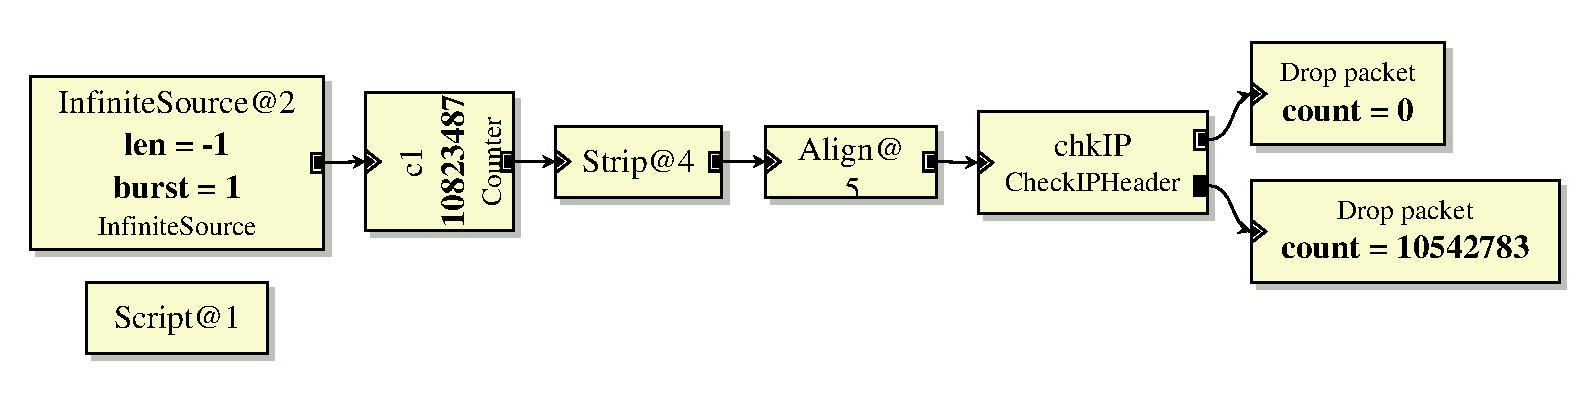
\includegraphics[scale=0.6]{counter_test.pdf}
	  \captionof{figure}{\texttt{Counter\_test} Click configuration}
	  \label{fig:countertest}
  \end{center}
  To avoid IP CRC checking, we temporarily disable CRC checking by using flag "\texttt{CHECKSUM false}" in \texttt{CheckIPHeader} element. Another solution is to use \texttt{SetIPChecksum} to repair CRC in generated IP packets. Since we can visualize the result by using \texttt{clicky} to replace steps that print out screen counting results from \texttt{Counter} elements. 
  \subsection{\texttt{RandInfiniteSource} element}
  \textbf{Location:} \texttt{elements/randinfinitesource.*} \\
  This element is implemented by modifying source of \texttt{InfiniteSource} element. Its function is similar to \texttt{InfiniteSource}, but by adding one more keyword (\texttt{RNDBYTEID}), generated packets may have random byte value at a specified position in payload. The idea of implementation is that before pushing out packets to the output port, packet payload is changed. Originally, data packet is already prepared one time by \texttt{setup\_packet} function before \texttt{InfiniteSource} releases packets. To make new element work, after modifying data, \texttt{setup\_packet} function should be called, otherwise generated packets do not change their content. Figure \ref{fig:test-randsource} shows the result of using \texttt{RandInfiniteSource} element to generate five packets with random value at the first byte.
  \begin{center}
	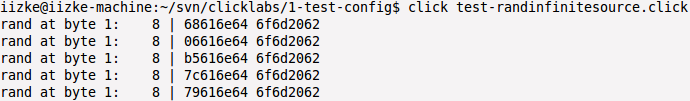
\includegraphics[width=0.9\textwidth]{test-randinfinitesource.png}
	\captionof{figure}{Test \texttt{RandInfiniteSource} element with 5 packets and random at the first byte}
	\label{fig:test-randsource}
  \end{center}

  \subsection{\texttt{RandomQueue} element}
  There are two ideas of implementing Random Queue:
  \begin{itemize}
  	\item Random at input: Pushing packets at random positions in queue, but pulling out packets as FIFO queue. We try to simulate this behavior by using built-in Click elements.
  	\item Random at output: Pushing packets in type of FIFO, but pulling out random packets in queue. We have implemented new element called \texttt{RandomQueue}.
  \end{itemize}
  To test our element, we first generate a high rate packet at input, store current timestamps, let packet go through our elements to output which has lower rate than the input. We then print out packet timestamps to see whether they are random or not.
  \subsubsection{Using built-in Click elements (compound element)}
  \textbf{Location:} \texttt{1-test-config/randomqueue.click} \\
  We have implemented two versions:
  \begin{itemize}
  	\item \texttt{BRandomQueue} (we call it Binary Random Queue): \texttt{MixedQueue} allows us to put packets in type of FIFO (input port 0) or LIFO (input port 1). Based on this function, input packets are put randomly (by \texttt{RandomSwitch} element) in either FIFO or LIFO input port. By this way, if queue size is $n$, there are $2^n^-^1$ possibilities created over total possibilities $(n!)$. Technical issue: "When full, \texttt{MixedQueue} drops incoming FIFO packets, but drops the  oldest  packet to make room for incoming LIFO packets". It means that at that time, when observing at output, we only see packets with increasingly timestamp, no randomly. We resolve this problem by writing a script to drop LIFO packet when queue is full.
  	\item \texttt{2PRandomQueue} (Two Partition Random Queue): We expand the above idea with two queues and using Stride scheduler to join them to the output. Note that, dropped packets in the first queue are push to the second queue.
  \end{itemize}
  \begin{figure}[ht]
      \centering
      \subfloat[\texttt{BRandomQueue}]{
      \label{fig:brandomqueue}
      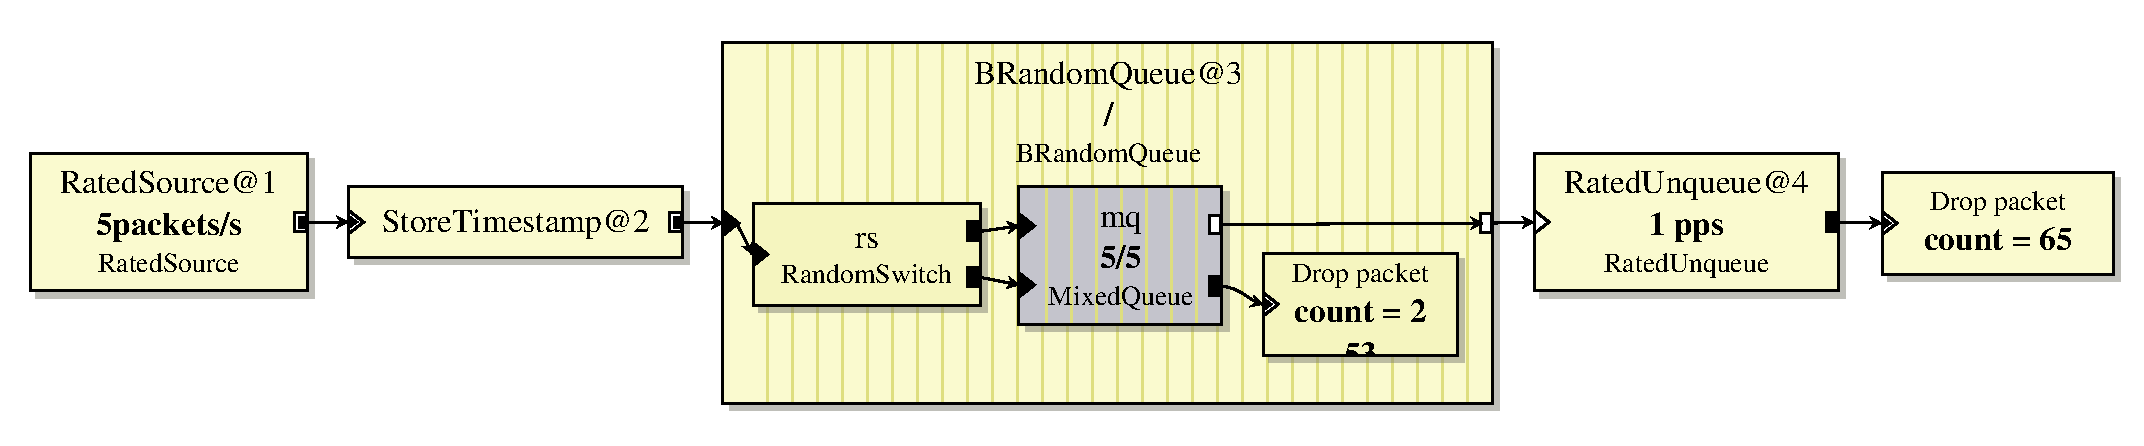
\includegraphics[width=0.8\textwidth]{brandomqueue.pdf}}
      
      \subfloat[\texttt{2PRandomQueue}]{
      \label{fig:2prandomqueue}
      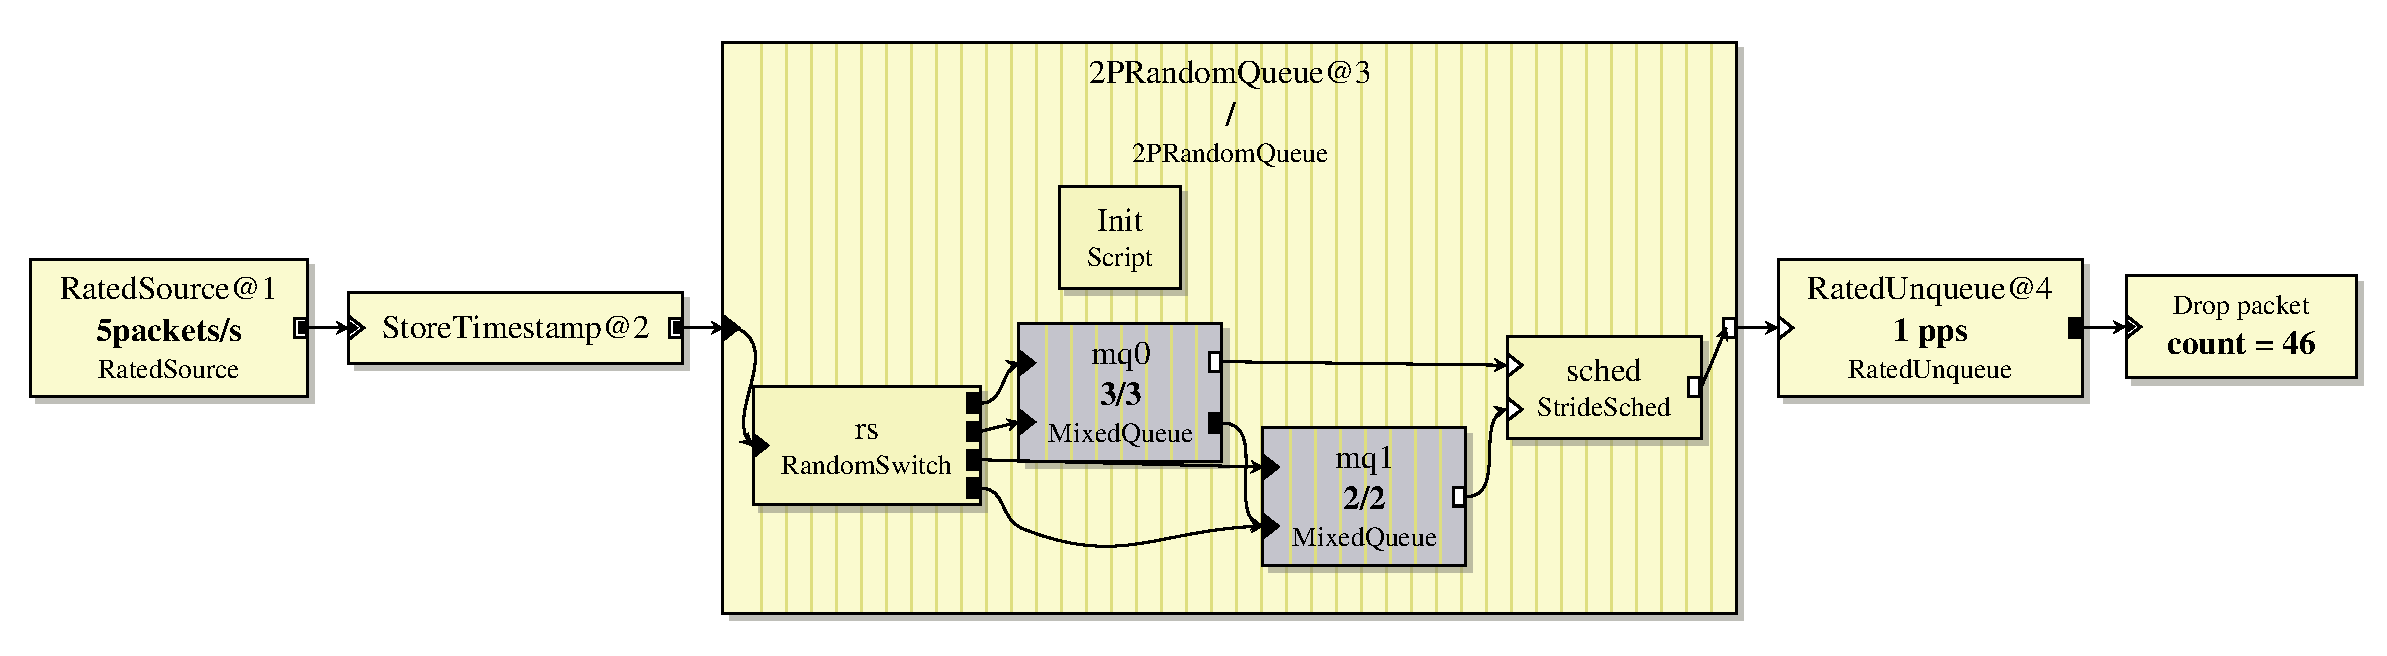
\includegraphics[width=0.8\textwidth]{2prandomqueue.pdf}}
      
      \caption{Random Queue configurations based on built-in Click elements}
      \label{fig:clickrandomqueue}
  \end{figure}
  Figure \ref{fig:test-clickrandomqueue} shows the result of testing these compound elements. The eight-byte number in each line is the timestamp of packet. We can see that this value does not increasing but randomly. 
    \begin{figure}
      \centering
      \subfloat[\texttt{BRandomQueue}]{
      \label{fig:test-brandomqueue}
      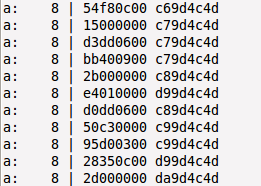
\includegraphics[width=0.35\textwidth]{test-brandomqueue.png}}      
      \subfloat[\texttt{2PRandomQueue}]{
      \label{fig:test-2prandomqueue}
      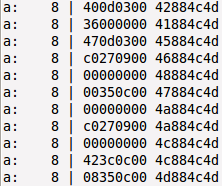
\includegraphics[width=0.3\textwidth]{test-2prandomqueue.png}}
      \caption{Test results of Random Queue configurations}
      \label{fig:test-clickrandomqueue}
  \end{figure}
  
  \subsubsection{Writing new element: \texttt{RandomQueue}}
  \textbf{Location:} \texttt{elements/randomqueue.*} \\
  This element is inherited from \texttt{ThreadSafeQueue} class. We reuse all the source code but modifying the \texttt{pull} function to make it pull out packets randomly. Since queue data structure is not suitable for pulling out random packet (only good for the head and tail packets), we use a trick that swapping between the random packet and the first packet. Step by step in our algorithm as following:
  \begin{center}
	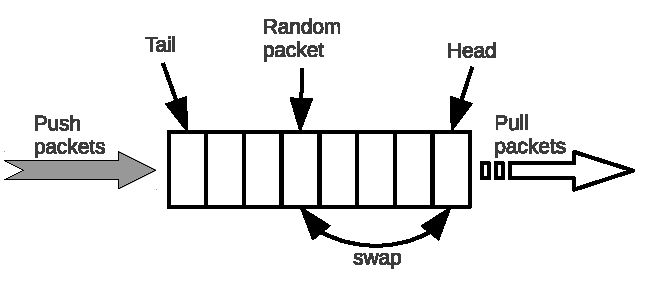
\includegraphics[scale=0.80]{randomqueue-alg.pdf}
	\captionof{figure}{Behavior of \texttt{RandomQueue} element}
	\label{fig:randomqueue}
  \end{center}

  \begin{itemize}
  	\item First, determining which packet is pulled out by a random number in the range from $0$ to \texttt{RandomQueue.length}.
  	\item Next, swapping the random packet and the first packet.
  	\item Last, pull out the first packet (but actually the random packet).
  \end{itemize}
  Figure \ref{fig:test-randomqueue} shows the result of testing \texttt{RandomQueue} element. The eight-byte number in each line is the timestamp of packet. We can see that this value does not increasing but randomly. It means this element works well.
  \begin{center}
	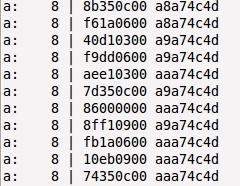
\includegraphics[scale=0.70]{test-randomqueue.png}
	\captionof{figure}{Test \texttt{RandomQueue} element}
	\label{fig:test-randomqueue}
  \end{center}

  \subsection{\texttt{Random\_IP\_generator} configuration}
  \textbf{Location:} \texttt{1-test-config/Random\_IP\_generator.click} \\
  We combine \texttt{RandInfiniteSource, RandomQueue} with other elements to build this configuration:
  \begin{itemize}
   	\item \texttt{RandInfiniteSource}: generate packets with random source IP address in the form 192.168.1.x. In this situation, we set up "RNDBYTEID 30".
   	\item \texttt{RandomQueue}: pull out packets at random position in queue. We can replace \texttt{RandomQueue} to another types of queue, such as FIFO or LIFO, by using \texttt{MixedQueue} element (comment lines in \texttt{Random\_IP\_generator} configuration). 
   	\item \texttt{SetCRC32, CheckCRC32}: set or check CRC32.
   	\item \texttt{RandomBitError}: to simulate an error free link via a queue element.
   	\item \texttt{Script}: we add some scripts to check states: 
       	\begin{itemize}
       		\item \texttt{autoupdate\_lostp\_estimation}: calculation of expected lost packets over input packets, based on bit error from \texttt{RandomBitError} and number of 'input' packets (\texttt{c1} in figure \ref{fig:randomipgenerator}).
       		\item \texttt{autoupdate\_real\_bit\_error}: real bit error cbased on \texttt{c1, c2}. 
       		\item \texttt{autoupdate\_lostp\_percent}: real lost packets over input packets based on \texttt{c1, c2}.
       	\end{itemize}
   \end{itemize} 
  \begin{center}
	  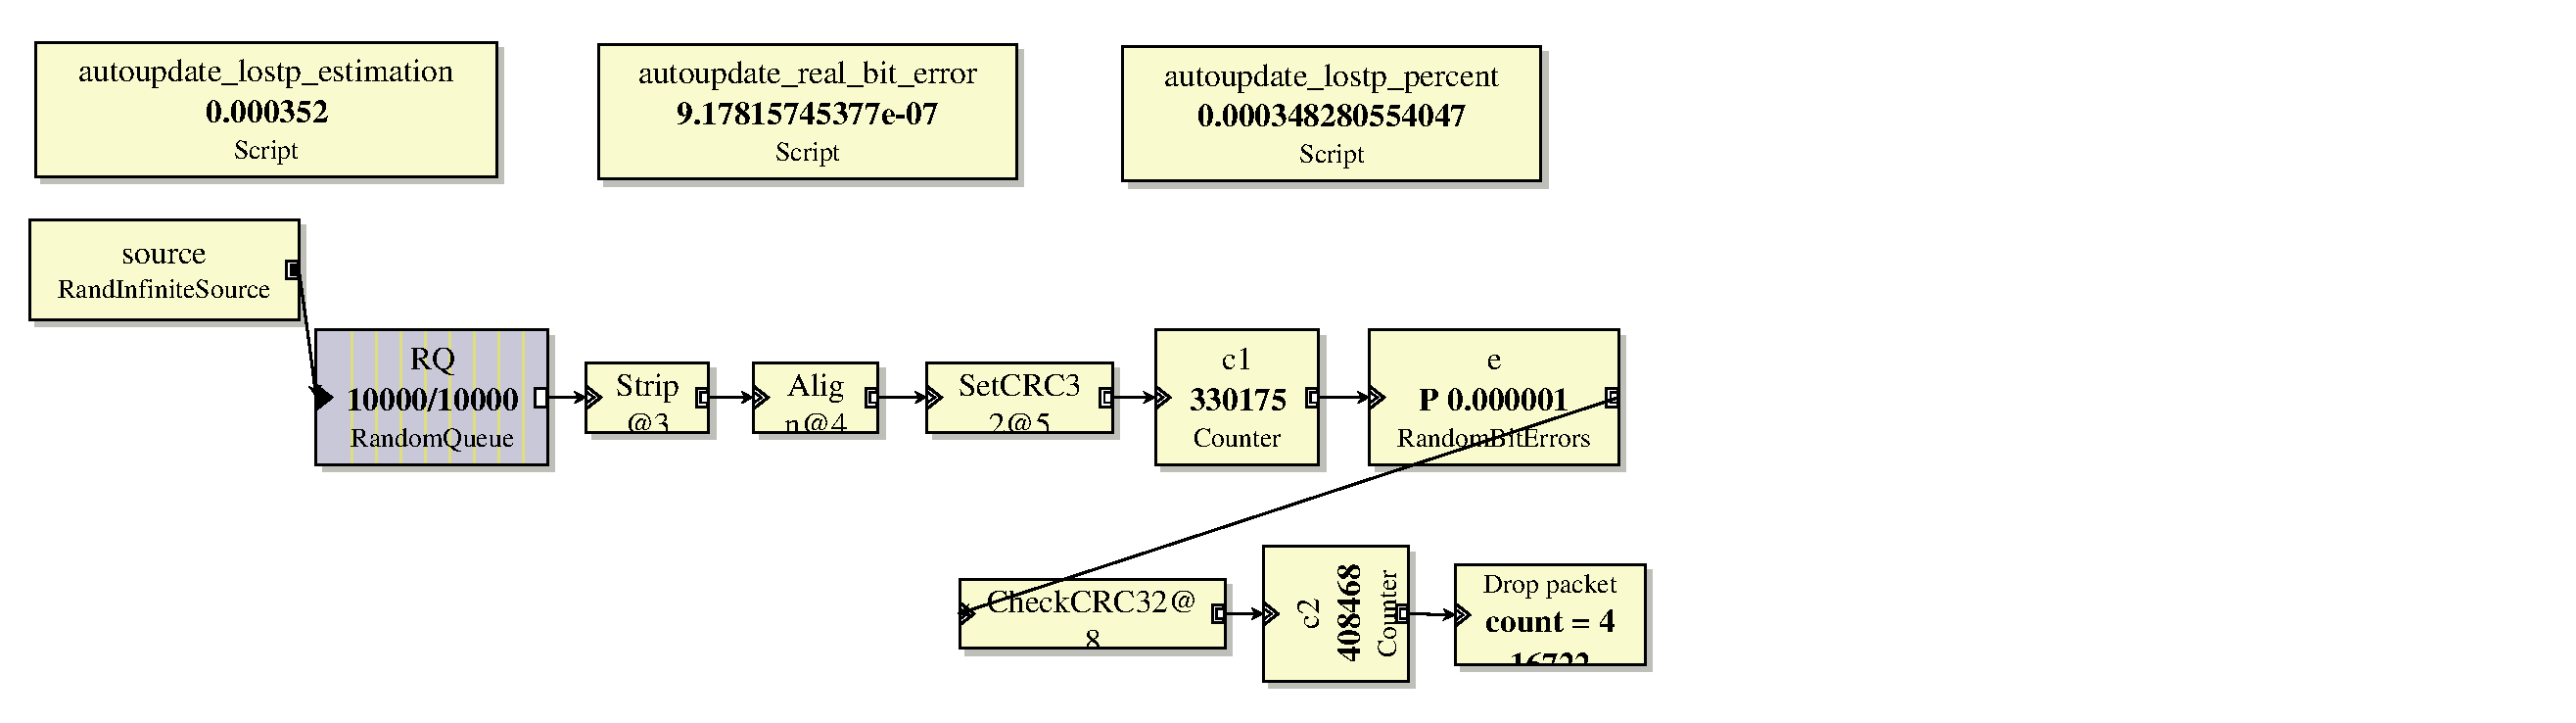
\includegraphics[scale=0.55]{Random_IP_generator.pdf}
	  \captionof{figure}{\texttt{Random\_IP\_generator} configuration}
	  \label{fig:randomipgenerator}
  \end{center}
  \section{TCP/UDP traffic generation}
  \subsection{TCP traffic}
  \textbf{Location:} \texttt{2-tcp-udp-generation/TCP\_Source.click} \\
  The procedure of generating TCP packet as following:
  \begin{itemize}
  	\item First, we use \texttt{TimedSource} to generate TCP packet without IP header.
  	\item After that, this packet is encapsulated IP header by \texttt{IPEncap}. Remember to setup "PROTO 0x06" to say that it is TCP packet.
  	\item Encapsulate ethernet header with "ETHERTYPE 0x0800" in each packet.
  \end{itemize}
  \begin{center}
	  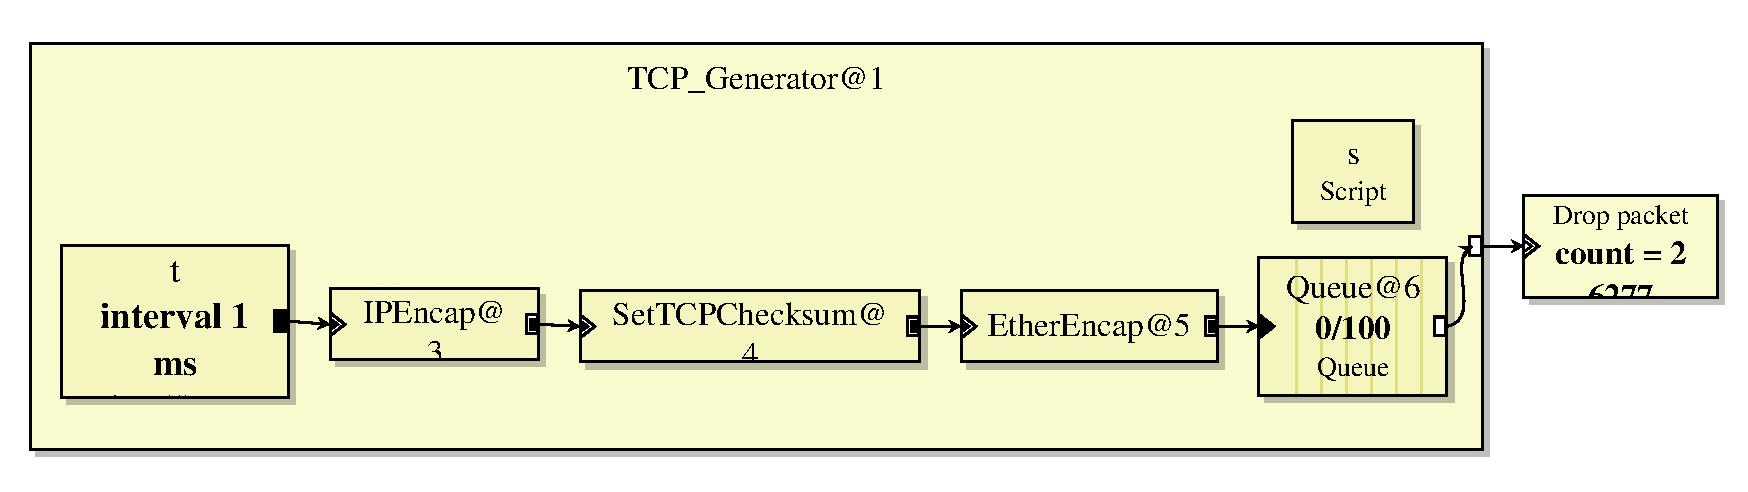
\includegraphics[scale=0.55]{TCP_Source.pdf}
	  \captionof{figure}{\texttt{TCP\_Source} element}
	  \label{fig:tcpsource}
  \end{center}
  \subsection{UDP traffic}
  \textbf{Location:} \texttt{2-tcp-udp-generation/UDP\_Source.click} \\
  \texttt{UDP\_Generator} operates like \texttt{TCP\_Generator}. Note: when using \texttt{IPEncap}, setup "PROTO 0x11" for UDP packet.
    \begin{center}
	  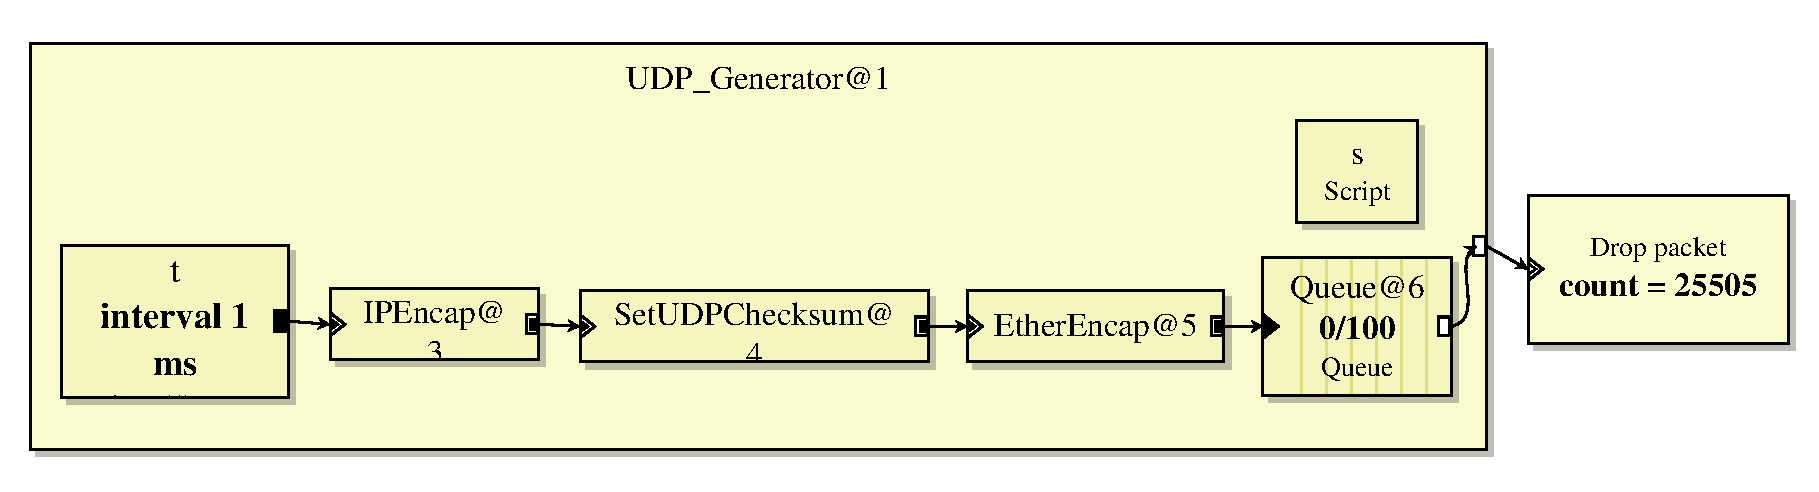
\includegraphics[scale=0.55]{UDP_Source.pdf}
	  \captionof{figure}{\texttt{UDP\_Source} element}
	  \label{fig:udpsource}
  \end{center}
  \subsection{\texttt{TCP\_UDP\_generator} configuration}
  \textbf{Location:} \texttt{2-tcp-udp-generation/TCP\_UDP\_generator.click} \\
  We build this configuration as in figure \ref{fig:tcpudp}. TCP source is created with rate about 1000 packets per second (pps) while UDP packet rate is 1 pps. Both sources are connected to a Round Robin scheduler (\texttt{rrsched}). Script \texttt{autoupdate\_scale} is used to check online the ratio between number of TCP packets and number of UDP packets. We see that this generator works well when both queues are not full or speed of output link (\texttt{TimedSink}) is very fast. When queues are full, the expected ratio is not guaranteed. At our observation, we try to formalize the ratio as following:
  \begin{itemize}
  	\item Let $r_{tcp}$, $r_{udp}$, $r$ are respectively the rate of TCP source, UDP source and output link. Let $ratio$ is the ratio between number of TCP packets over number of UDP packets at output link.
  	\item Let $R = (r_{tcp} + r_{udp})$, and $m = \min(r_{tcp}, r_{udp})$.
  	\item If $r \ge R$: $ratio \to \frac{r_{tcp}}{r_{udp}}$
  	\item If $r \le 2m$: $ratio \to 1$
  	\item If $ 2m < r < R$: $ratio \to \frac{m}{r - m}$
  \end{itemize}
  In general, we have a formular of ratio like: $ratio = \frac{m}{\min(R, \max(2m, r)) - m}$.
    \begin{center}
	  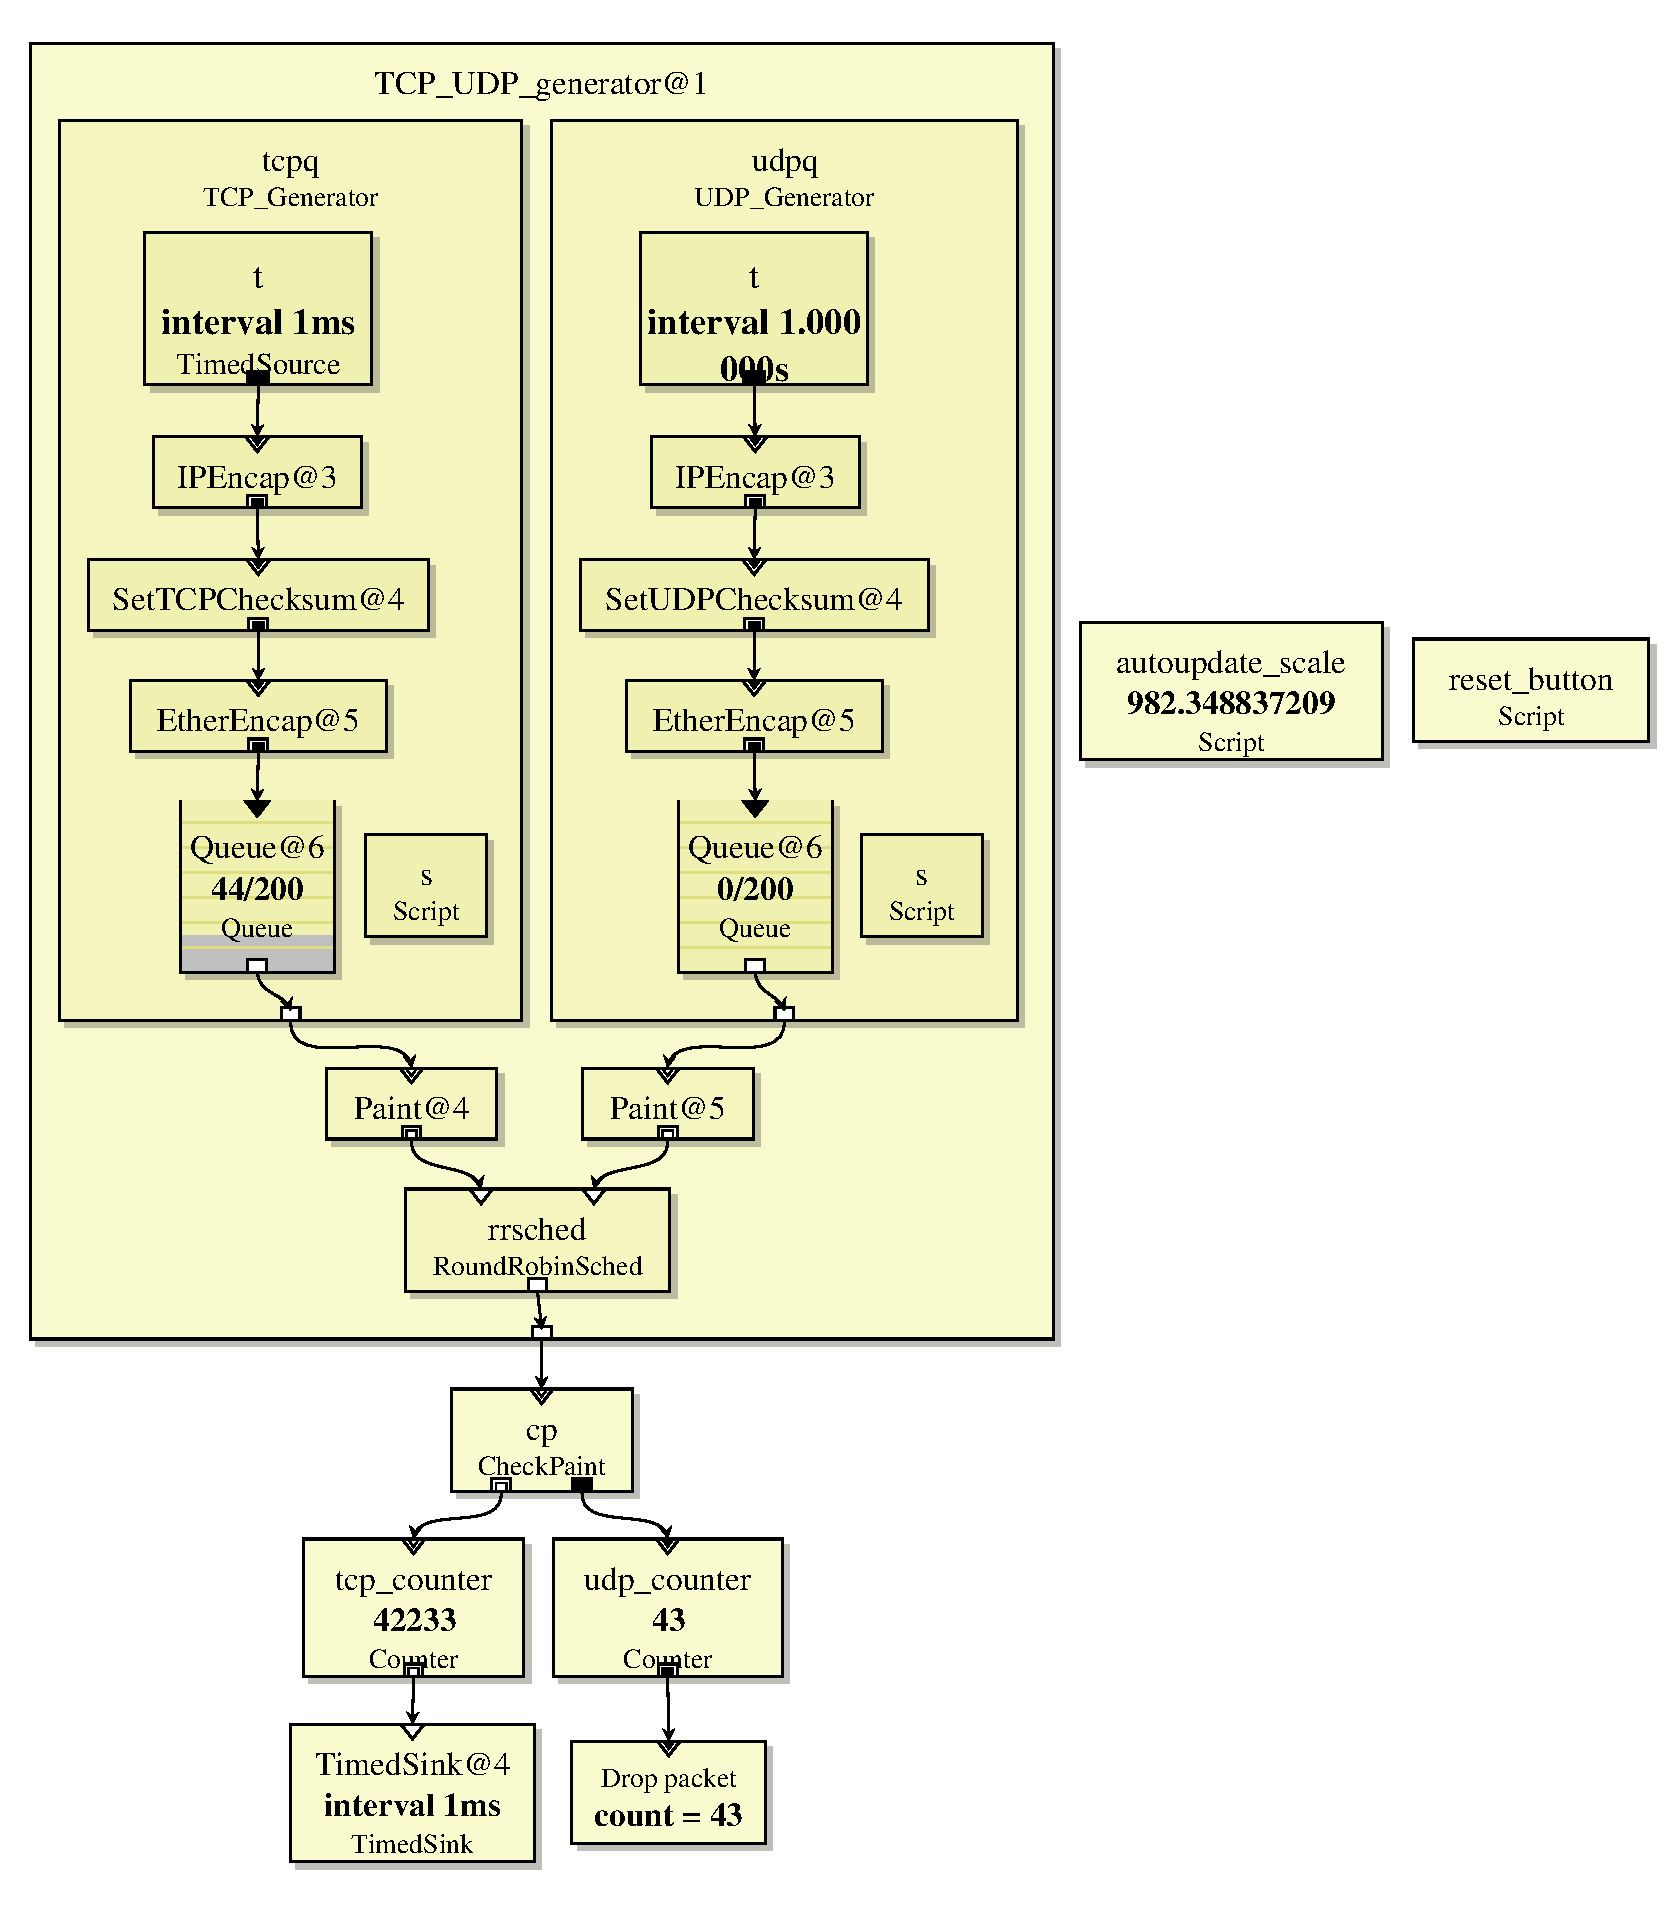
\includegraphics[scale=0.4]{TCP_UDP_generator.pdf}
	  \captionof{figure}{\texttt{TCP\_UDP\_generator} configuration}
	  \label{fig:tcpudp}
  \end{center}
  \section{Shapers and Policers}
  In this part, we implement elements with consideration at packet level, not byte level.
  \subsection{Uncontrolled flow}
  \textbf{Location:} \texttt{3-shaper-policer/uncontrol-flow.click} \\
  We have tried some implementations of uncontrolled flow but the main idea is that the inter-time (interval) between two consecutive packets is a random
  number. All implementations of uncontrolled flow are put in \texttt{3-shaper-policer/uncontrol-flow.click}. Normally, we use \texttt{RatedSource} or \texttt{TimedSource} to generate packets at a specific rate. After some time, we use Script to change their rate or interval at a random values. We list here with a few lines of description of each implementation:
  \begin{itemize}
  	\item \texttt{UncontrolledFlow0}: We use two rated sources, one for generating regular rated source, one for generating burst. These sources are connected to a pull switch to choose from which source packets are generated. At any time generating packets, we choose a source to generate next packets through a script. 
  	\item \texttt{UncontrolledFlow1}: Only one source (\texttt{InfiniteSource}) is used and connected directly to the output. We used another two scripts named \texttt{change\_rate} and \texttt{autoupdate\_change\_burst} to change rate and burst duration at runtime.
  	\item \texttt{SimpleUncontrolledFlow}: we use \texttt{RatedSource} instead of \texttt{InfiniteSource} and one script to change the rate of source. This script operates in type ACTIVE and period of one second.
  	\item \texttt{ProbUncontrolledFlow} (Figure \ref{fig:probuncontrolledflow}): similar to \texttt{SimpleUncontrolledFlow} but change-rate script operates in type PACKET. When one packet go through this script, it will decide whether rate of source is changed or not based on a probability defined by user.
  	\item \texttt{BurstUncontrolledFlow}: We use eight sources (\texttt{RatedSource}) generating packets in the same rate, all connected to a \texttt{ThreadSafeQueue}. In each source, packets can be dropped at a defined probability. As a result, this compound element generates packets at a particular rate but random burst duration (maximum is 8). 
  \end{itemize}
  \begin{center}
	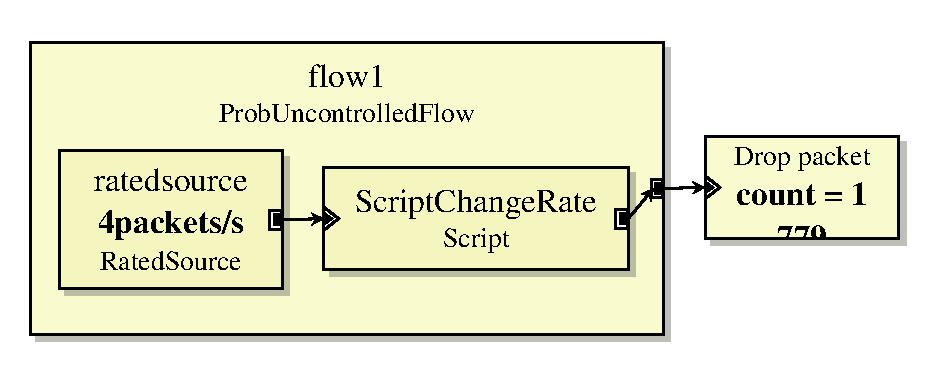
\includegraphics[width=0.60\textwidth]{probuncontrolledflow.pdf}
	\captionof{figure}{Uncontrolled flow with probability of changing rate source.}
	\label{fig:probuncontrolledflow}
  \end{center}
  
  \subsection{Leaky bucket}
  \textbf{Location:} \texttt{3-shaper-policer/leaky-bucket.click} \\
  Since leaky bucket does not admit any burtiness, we design the leaky bucket policer with a queue of size one (maximum one packet in a queue at a time) (figure \ref{fig:test-leaky}). After that, we use \texttt{RatedUnqueue} or \texttt{TimedSource} to create CBR source. We use both these elements because of a technical issue: when the rate is less than 1000 packets/second, \texttt{RatedUnqueue} can release packets from queue with burstiness. So, at the beginning of starting leaky policer, the \texttt{Init} script will decide which one of unqueue elements is used.
  \begin{center}
	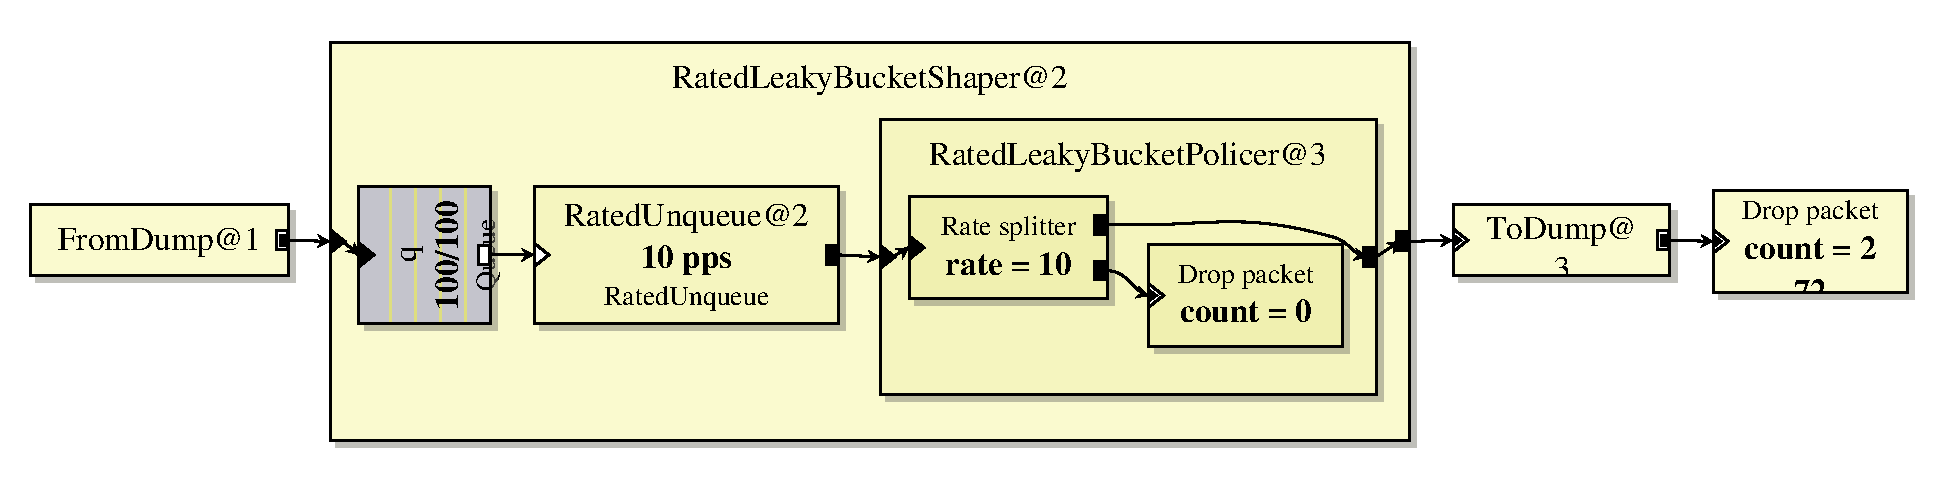
\includegraphics[width=1.0\textwidth]{leaky-shaper.pdf}
	\captionof{figure}{Leaky bucket configuration (policer and shaper)}
	\label{fig:test-leaky}
  \end{center}
  Scenario of testing leaky bucket: \texttt{ProbUncontrolledFlow} is the source of packets with maximum rate 1000 pps (packets per second). The leaky policer only allows 400 pps. Shaper of leaky bucket uses a buffer of 2000 packets and generate packets from buffer at rate 400pps to the leaky policer. Figure \ref{fig:test-leakypolicer-graph} shows that the number of output packets is linear to time although the input is not.  
  \begin{center}
	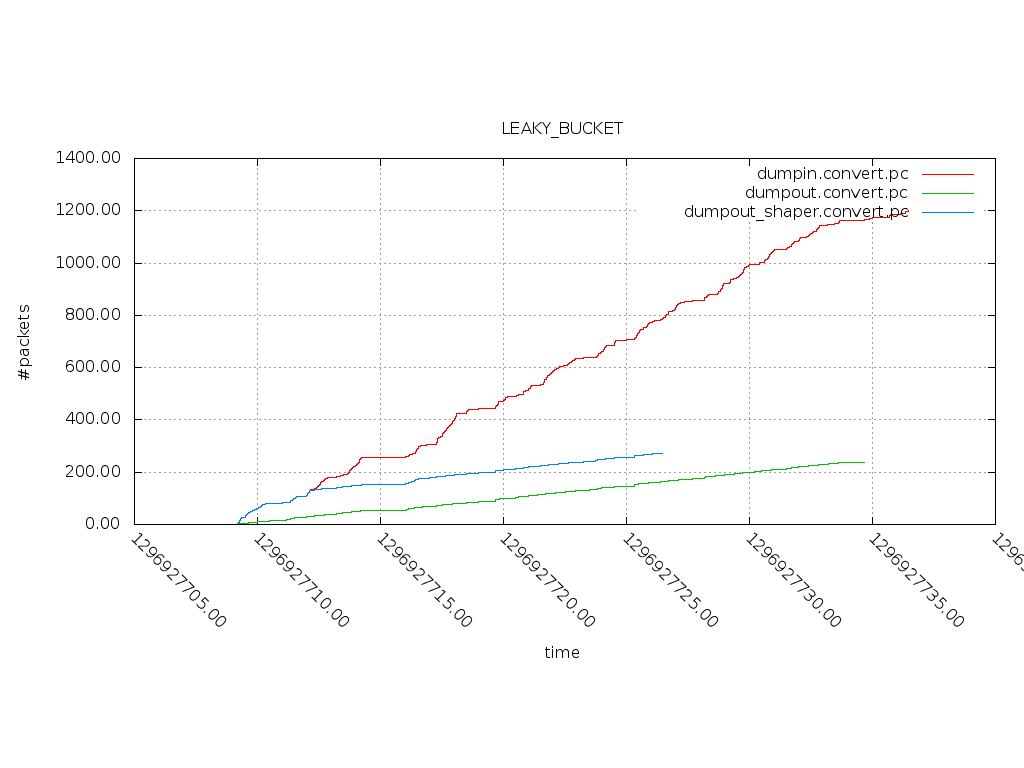
\includegraphics[width=0.8\textwidth]{leaky-count.png}
	\captionof{figure}{Monitor number of packets at input (uncontrolled flow) and output of leaky policer and shaper}
	\label{fig:test-leakypolicer-graph}
  \end{center} 
  
  \subsection{Token bucket}
  \textbf{Location:} \texttt{3-shaper-policer/token-bucket.click} \\
  Token bucket is designed similar to leaky bucket but expand the size of queue as a number of burst duration, see \texttt{RatedTokenBucketPolicer3} in figure \ref{fig:test-token}. But before implementing this element, there are some alternative implementations which are more complex:
  \begin{itemize}
  	\item \texttt{RatedTokenBucketPolicer1}: We use a variable-size queue in this element. The size of queue is increased with the rate that is equal to the rate of token bucket. Each time a packet goes out of queue, size of queue is decreased one. To allow repeating burst at any periodic interval time, this element uses flag REPEATED.
  	\item \texttt{RatedTokenBucketPolicer2}: This element uses a sample source (same rate as token bucket, operating as a \textit{token generator}) and two counters counting the number of output packets ($CO$) and the number of generated token packets ($CT$). This element guarantees that at any time, \\ 
  	\begin{align*}CO \le CT \le CO + burst\_duration \end{align*}
  	If it is satisfied, input packets are pushed to output immediately, otherwise they are dropped. This element releases packets to output as soon as possible (no queue is needed to store input packets) while other implementations try to store input packets first and then regulate the output flow at a given rate.
  \end{itemize} 
  \begin{center}
	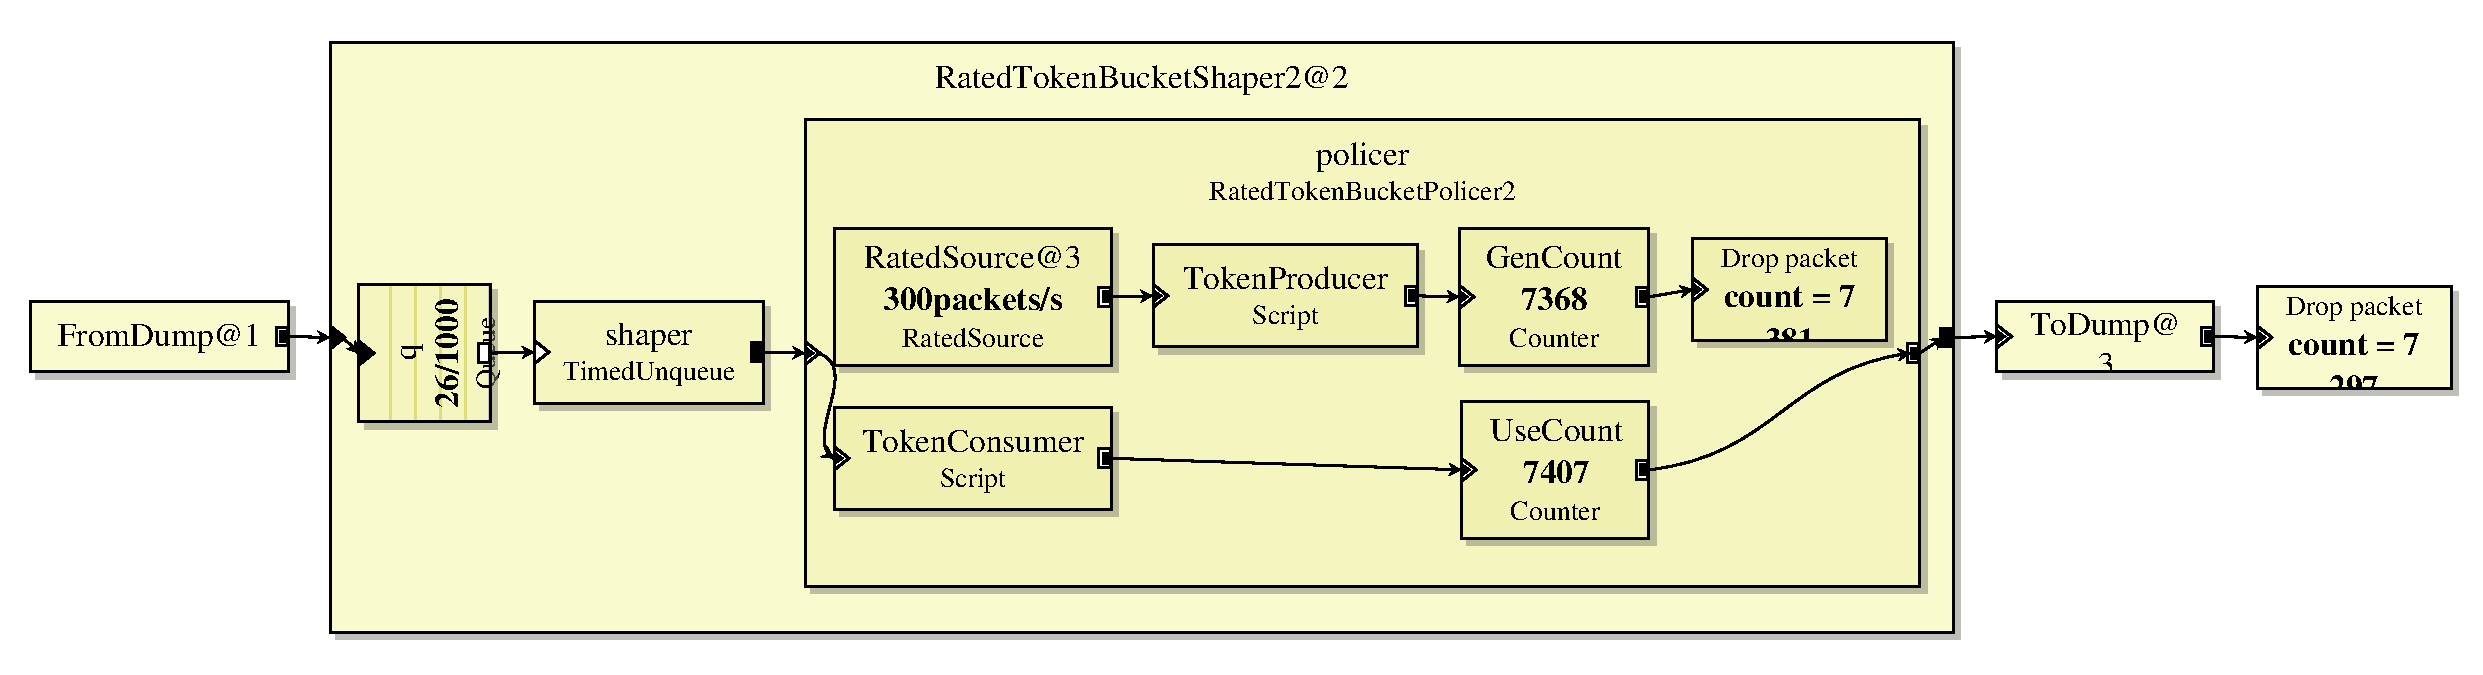
\includegraphics[width=0.8\textwidth]{token-shaper.pdf}
	\captionof{figure}{Token bucket configuration \texttt{RatedTokenBucketShaper3}}
	\label{fig:test-token}
  \end{center}
  
  \begin{center}
	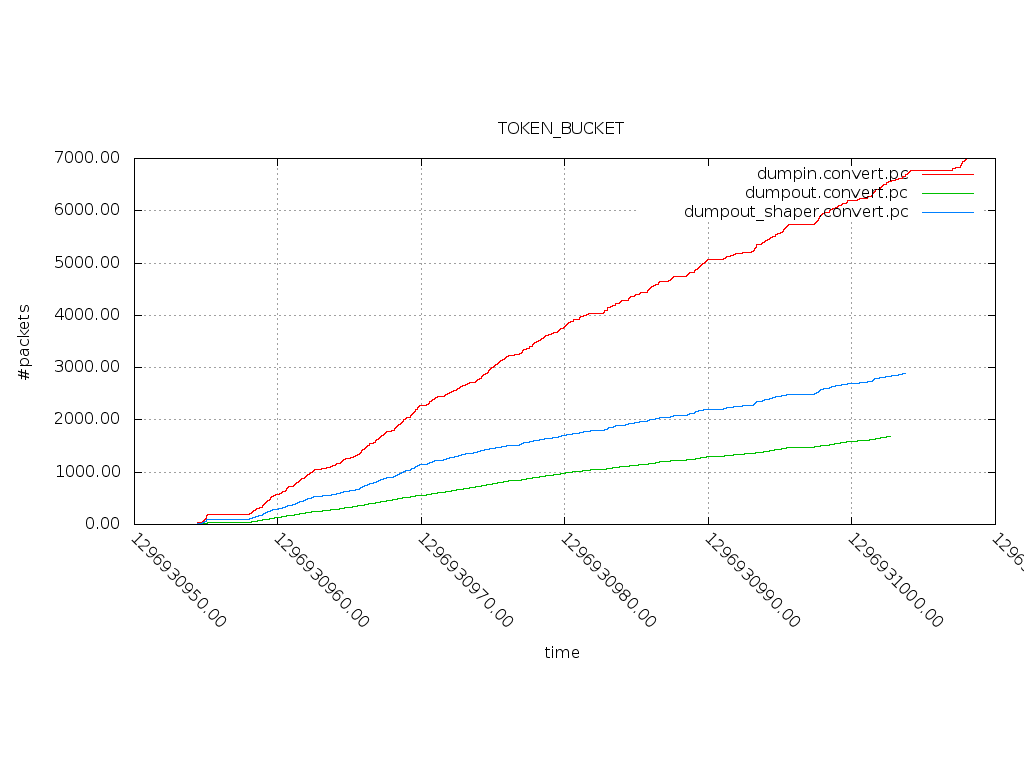
\includegraphics[width=0.7\textwidth]{token-count.png}
	\captionof{figure}{Number of packets at input (uncontrolled flow) and output of token policer and shaper}
	\label{fig:test-tokenpolicer-graph}
  \end{center} 

  Figure \ref{fig:test-token-leaky-graph} does a comparison of token and leaky bucket. The scenario is: we try to regulate a \texttt{BurstUncontrolledFlow}  (rate is 1 pps and maximum burst is 8) by a token and a leaky bucket policer. Token bucket policer is \texttt{RatedTokenBucketPolicer3} (rate is 10 pps, burst is 10), and leaky policer is \texttt{RatedLeakyBucketPolicer} (rate is 10 pps). We see that token policer can allow some burst duration but leaky policer limits it.
  \begin{center}
	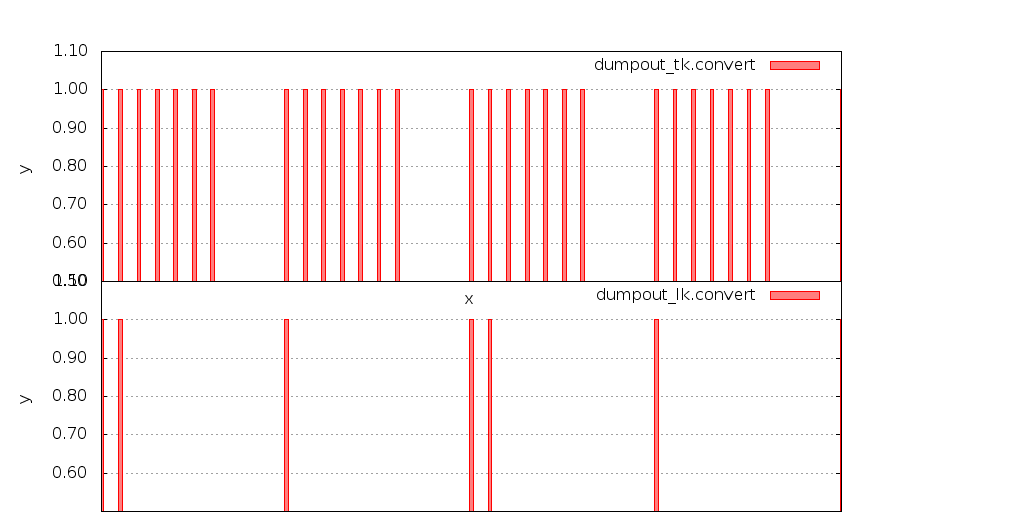
\includegraphics[width=0.7\textwidth]{compare-lk-tk.png}
	\captionof{figure}{Comparision of Token bucket and Leaky bucket}
	\label{fig:test-token-leaky-graph}
  \end{center} 
  
  \subsection{Negotiation (CIR, CBS, EBS)}
  \textbf{Location:} \texttt{3-shaper-policer/negotiation.click} \\
  Figure \ref{fig:negotiation2} shows one implementation of negotiation (\texttt{RatedNegotiablePolicer2}). The idea is: input packets are gone through \texttt{RatedLeakyBucketShaper} (with leaky rate $R_L = \frac{CIR * (CBS + EBS)}{CBS}$) and then gone through \texttt{RatedTokenBucketShaper2} (with token rate $R_T = CIR$ and burst duration is $EBS$). At output, we guarantee that in interval time $T = \frac{CBS}{CIR}$, maximum number of output packets is $(CBS + EBS)$ and flow is shapped to rate $CIR$ with a maximum burst duration $EBS$.   
  \begin{center}
	\includegraphics[width=0.80\textwidth]{negotiation2.pdf}
	\captionof{figure}{Implementation of \texttt{RatedNegotiablePolicer2}}
	\label{fig:negotiation2}
  \end{center}  
  We brieftly describe other implementations of negotiation which can be found in \texttt{negotiation.click} as following:
  \begin{itemize}
  	\item \texttt{RatedNegotiablePolicer1}: Input packets are stored in a queue with length $(CBS + EBS)$. At each interval $T = \frac{CBS}{CIR}$, all packets in queue are released. This implementation is simple with only one \texttt{TimedUnqueue} to control $T$, one Queue to do negotiation. To recognize high and low priority, at each packet, before storing it in queue, we check if queue length is larger than $CBS$ then its priority is low. However, this element is a non-work-conserving element, so we only consider it when $T$ is small (should be $T \le 1$, or the best case is $CBS = 1$).
  	\item \texttt{RatedNegotiablePolicer4}: See figure \ref{fig:negotiation4}. Input packets are classified into low and high priority. Packet is high priority and put into \texttt{HighQueue} if there is free space in \texttt{HighQueue} (capacity $CBS$), otherwise it is in \texttt{LowQueue} (capacity $EBS$) with low priority. Since rate $CIR$ is fixed, the window time $T = \frac{CBS}{CIR}$ is scale to $CBS$. We use a counter \texttt{TimeCount} to know when the window time is end (by observing $\texttt{TimeCount} = CBS$). If this happens, we reset all the counters for a new window time. Since we calculate the window time based on $CBS$, we have to make sure that there are always packets to \texttt{TimeCount} at rate $CIR$. So, \texttt{SampleSource} is used to generate packets at rate $CIR$ to guarantee that condition. Whenever there are no packets from \texttt{HighQueue}, the \texttt{PrioScheduler} will get packets from \texttt{SampleSource}. In the end, temporary packets will be removed before going to the output. The number of packets in a window time $T$ always less than or equal to $(CBS+EBS)$. The high priority packets are on port 0, and the low priority packets are on port 1. 
  \end{itemize}
  \begin{center}
	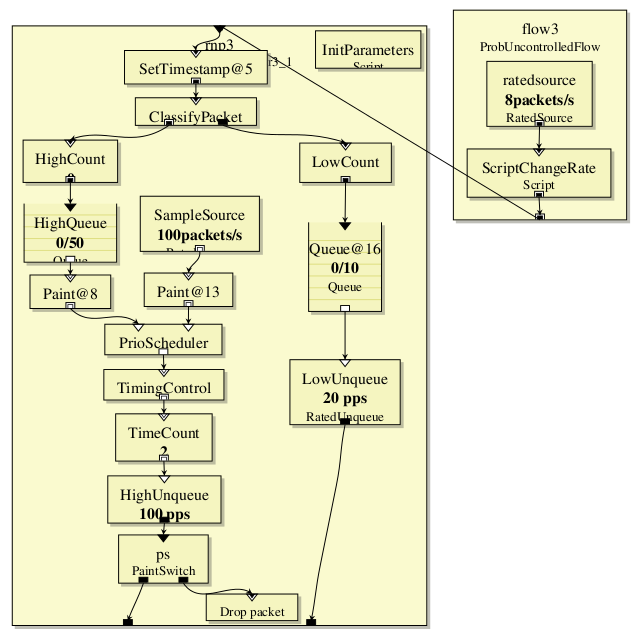
\includegraphics[width=0.80\textwidth]{negotiation.png}
	\captionof{figure}{Implementation of \texttt{RatedNegotiablePolicer4}}
	\label{fig:negotiation4}
  \end{center}
  We test \texttt{RatedNegotiablePolicer2} and \texttt{RatedNegotiablePolicer4} with an uncontrolled input source, maximum rate 500 pps. The negotiation is: CBS = 50, EBS = 10 and CIR = 100 (pps). Results are shown in figure \ref{fig:negotiation-test}. The red line (\texttt{dumpin2}) is representation of input flow. The green line (\texttt{dumpout2}) is represented to \texttt{RatedNegotiablePolicer2} and the other line of \texttt{RatedNegotiablePolicer4} (\texttt{dumpout4}). We can see that the number of output packets, in a window time $T = 0.5s$, is trimmed at 60 packets following the rules of negotiation, but line of (\texttt{dumpout4}) is a little higher than line of (\texttt{dumpout2}).
    \begin{figure}
    \centering
    \subfloat[Number of packets in a time interval $T=\frac{CBS}{CIR}=0.5s$]{
      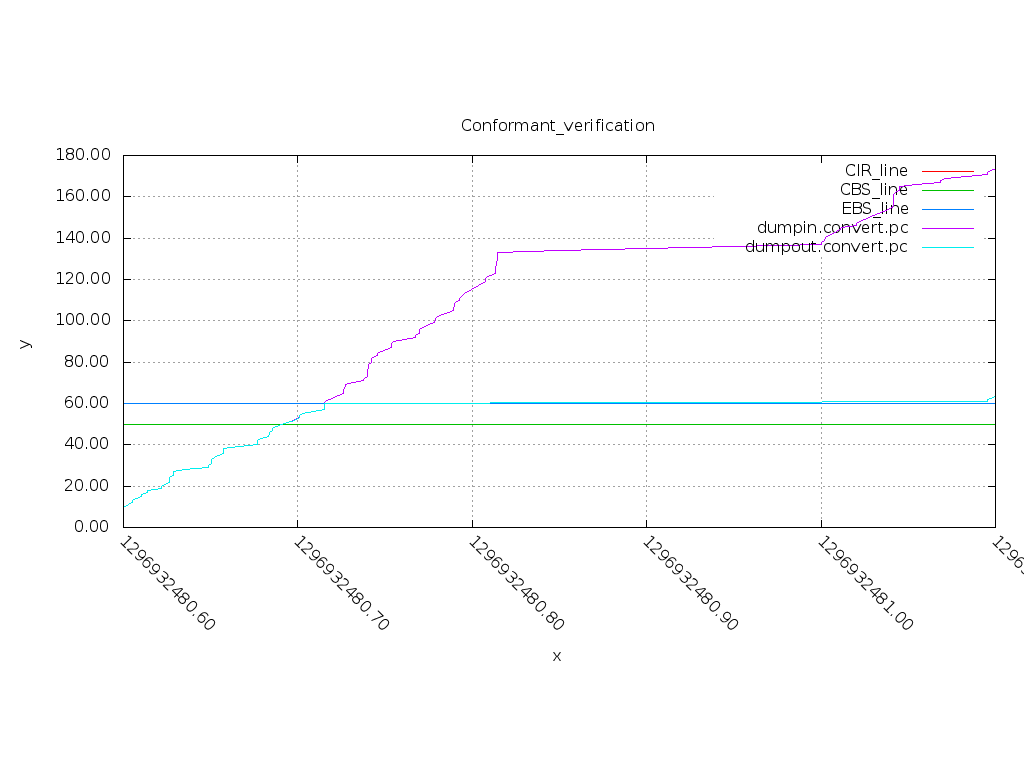
\includegraphics[width=0.55\textwidth]{negotiation-check.png}
	    \label{fig:negotiation-check}}
    \subfloat[Number of packets over time]{
      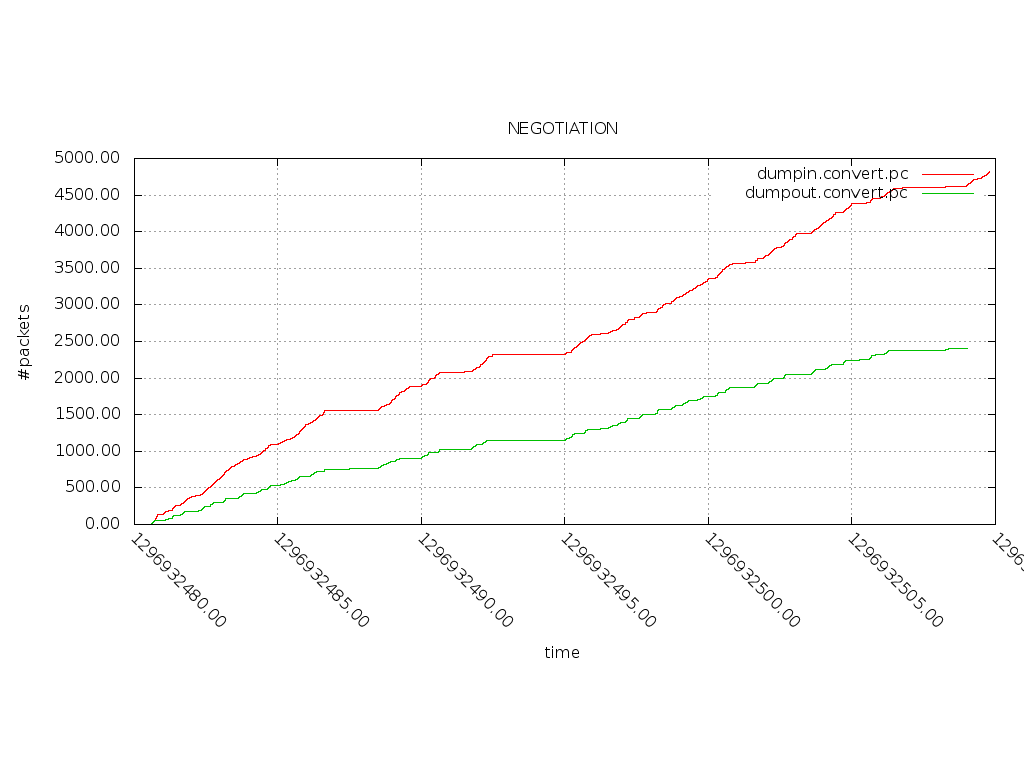
\includegraphics[width=0.55\textwidth]{negotiation-count.png}
	    \label{fig:negotiation-count}}
	    
	    \caption{Negotiation with \texttt{RatedNegotiablePolicer2} and \texttt{RatedNegotiablePolicer4}}
	    \label{fig:negotiation-test}
    \end{figure}

  \subsection{Generic Cell Rate Algorithm - GCRA}
  \textbf{Location:} \texttt{3-shaper-policer/gcra.click} \\
  GCRA configuration is in figure \ref{fig:gcra}. We implement this element by using \texttt{SetVirtualClock}. Element \texttt{SetVirtualClock} works as following (more details in section~\ref{section:virtualclock}): when a packet comes to this element, it will set this packet's timestamp annotation to a new value, and also remember the last theoritical cell arrival time ($TAT$). Before letting packets approach \texttt{SetVirtualClock}, packets have to go through script \texttt{CheckTime}. If packet comes too soon, it will be dropped, otherwise it will go to \texttt{SetVirtualClock} and make a new $TAT$. We test this element by a \texttt{ProbUncontrolledFlow} with maximum rate 10 pps. Our \texttt{GCRA} is set up to allow $TAT = 0.2$ and $\tau = 0$. In figure \ref{fig:test-gcra}, we plot the packet arrival time of input (lower part) and output and see that output flow is less dense than input flow, and the inter-time between packets is guaranteed. 

  \begin{center}
	\includegraphics[width=0.80\textwidth]{gcra1.pdf}
	\captionof{figure}{\texttt{GCRA} configuration}
	\label{fig:gcra}
  \end{center}
  
  \begin{center}
	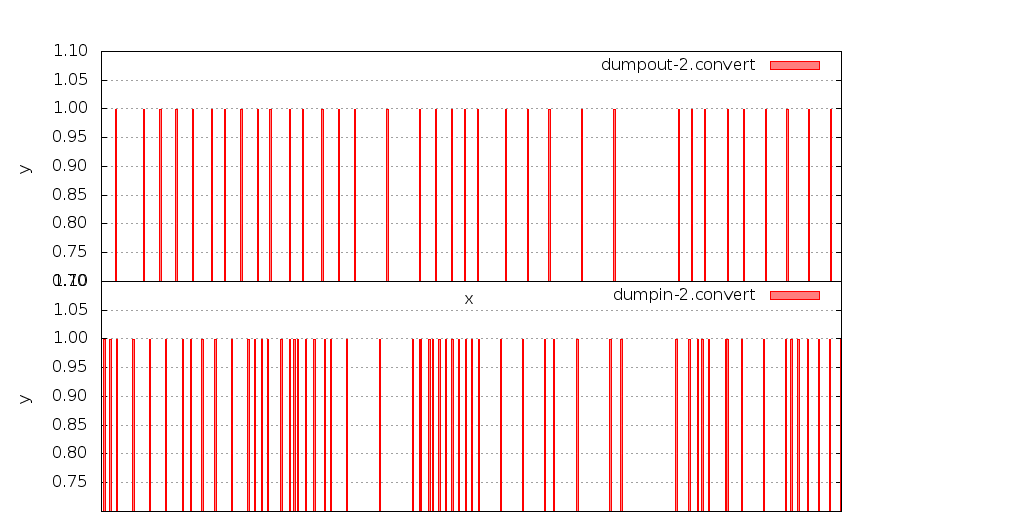
\includegraphics[width=0.80\textwidth]{test-gcra.png}
	\captionof{figure}{Testing GCRA configuration with flow \texttt{ProbUncontrolledFlow}}
	\label{fig:test-gcra}
  \end{center}
  
  \section{Schedulers}
  \subsection{FIFO scheduler}
  \textbf{Location}: \texttt{4-scheduler/FIFO\_Sched.click}\\
  There are two ways of building FIFO scheduler. The first and simple way is to use \texttt{ThreadSafeQueue} element. All inputs are connected into input of queue and output of queue is connected to output of FIFO scheduler. The second way is to use \texttt{TimeSortedSched} element to which all inputs connect through queues. We test our FIFO scheduler with three flows and their rate respectively 1 pps, 3 pps, 6 pps. FIFO scheduler only processes 1 pps. Figure \ref{fig:test-fifo} shows the result that the high rate flow (blue color - out2) makes a huge effect on the output link.
  \begin{center}
	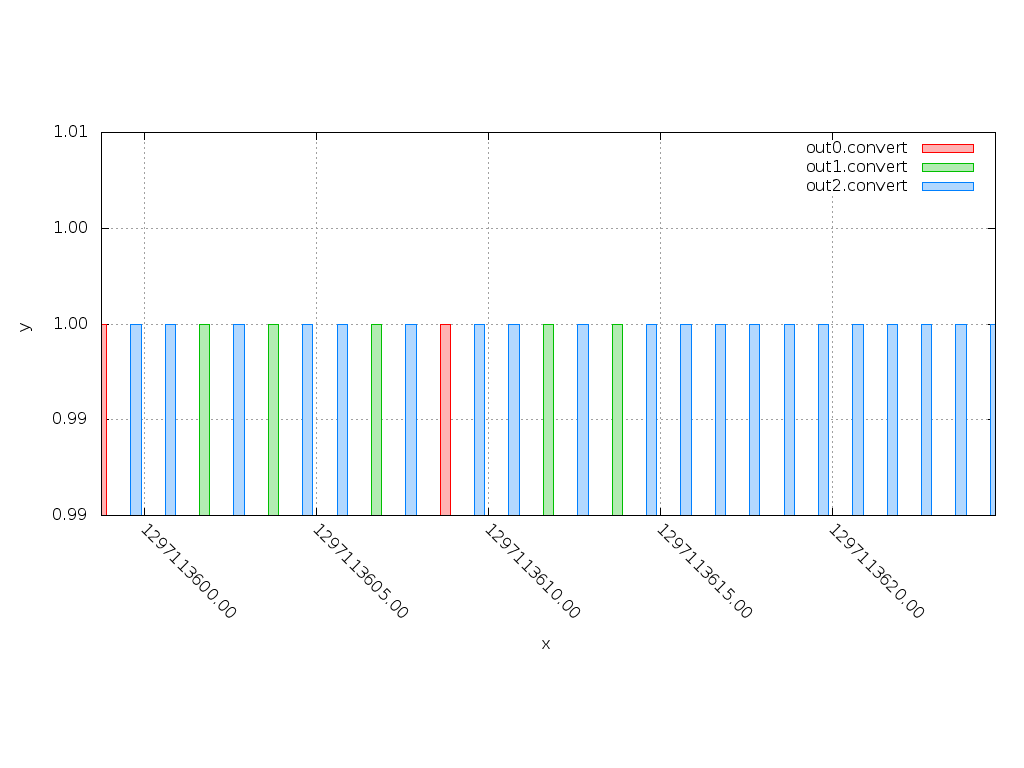
\includegraphics[height=0.3\textheight, width=0.70\textwidth]{fifo-dense.png}
	\captionof{figure}{Testing \texttt{FIFOSched} configuration}
	\label{fig:test-fifo}
  \end{center}
  
  \subsection{Round Robin scheduler}
  \textbf{Location}: \texttt{4-scheduler/RR\_Sched.click}\\
  Round Robin Scheduler is a built-in element in Click. We test this scheduler with the same scenario as described in testing FIFO scheduler. Although the inputs have diffirent rates, the output link is shared fairly to all three flows (figure \ref{fig:test-rr}) but it does not take care of packet's length.
  \begin{center}
	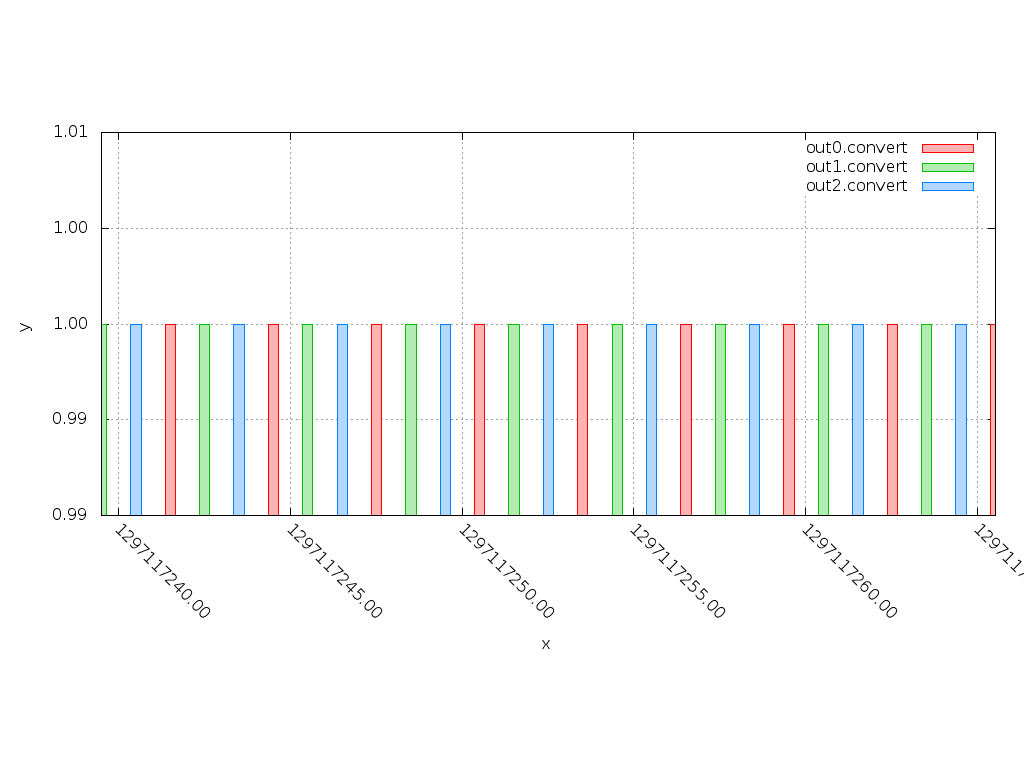
\includegraphics[height=0.3\textheight, width=0.70\textwidth]{rr-dense.png}
	\captionof{figure}{Testing \texttt{RRSched} configuration}
	\label{fig:test-rr}
  \end{center}
  
  \subsection{Deficit Round Robin scheduler}
  \textbf{Location}: \texttt{4-scheduler/DRR\_Sched.click}\\
  Deficit Round Robin (DRR) Scheduler is a built-in element in Click. We also test DRR scheduler with three flows, but the size of packets in each flow are 500, 1000 and 1500 bytes respectively. The result in figure \ref{fig:test-drr} shows that DRR scheduler guarantee bandwidth provided to each flow. The small-packet size flow is scheduled more times than other flows. When working with DRR scheduler and checking its source code, we know that the quantum byte is 500. It means for each round, deficit of each flow is increased 500. If we setup flows with too small in packet length, those flows will send out a lot of packets before next flows are scheduled to send packets. Or in contrast, flows having large size packets will wait for a long time before sending out packets.
  \begin{center}
	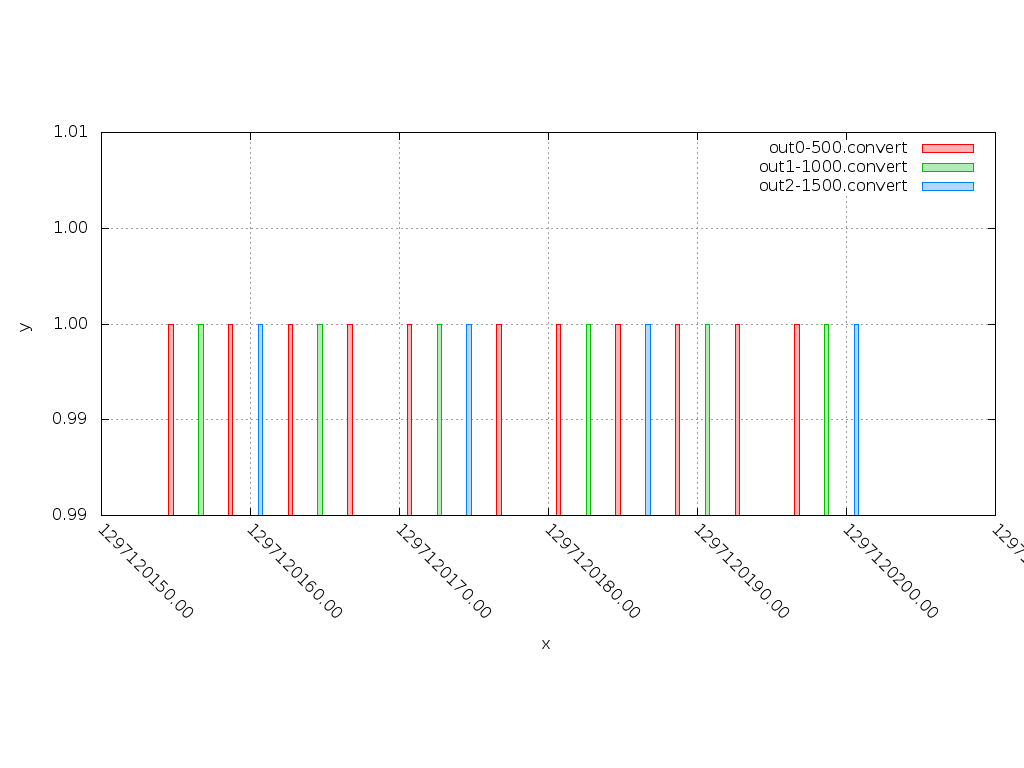
\includegraphics[width=0.70\textwidth]{drr-dense.png}
	\captionof{figure}{Testing \texttt{DRRSched} configuration}
	\label{fig:test-drr}
  \end{center}
  
  \subsection{Weighted Round Robin Scheduler}
  We implement this scheduler in two versions. The first is compound element that based on Round Robin scheduler. The second is a new element.
  \subsubsection{WRR scheduler - compound element}
  \textbf{Location}: \texttt{4-scheduler/WRR\_Sched.click}\\  
  This scheduler is based on Round Robin scheduler. The main idea is that: weight of each flow is scaled to number of ports assigned to that flow. A high weight flow will have more input ports of Round Robin scheduler. Figure \ref{fig:wrr-compound} is an example of WRR with two weights: 1 and 2. Source \texttt{s0} has weight 1 and connect to port 1 of \texttt{rrsched}. Source \texttt{s1}, weight 2, is provided two input ports (0 and 2) of \texttt{rrsched}. In practice, we need to take care of distribution of ports to have the fairness in response time. Besides, this approach also loses the sequence of packets in each flow. We build another WRR scheduler supporting three input flows with weight 1, 2 and 3 respectively. The result is shown in figure \ref{fig:test-wrr-compound} which presents the timestamp of packets at output link.
  \begin{center}
	\includegraphics[width=0.70\textwidth]{2wrr.pdf}
	\captionof{figure}{Configuration of \texttt{WRRSched} compound element with two input flows and weight 1, 2}
	\label{fig:wrr-compound}
  \end{center}

  \begin{center}
	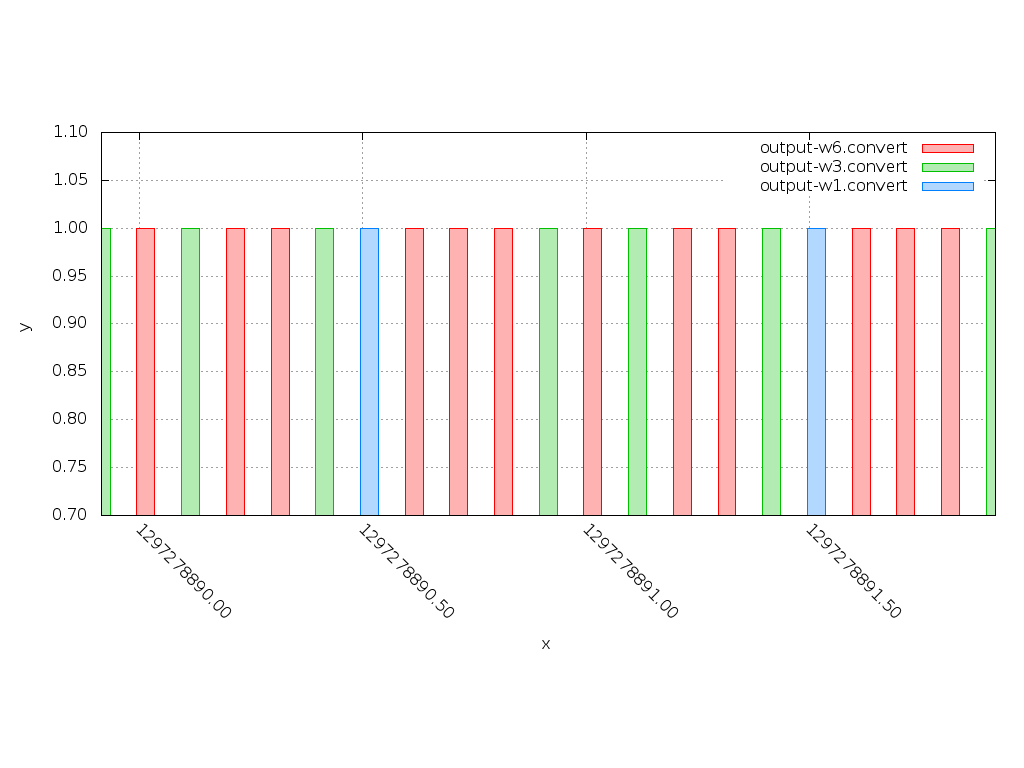
\includegraphics[width=0.70\textwidth]{wrr2-dense.png}
	\captionof{figure}{Testing \texttt{WRRSched} compound element}
	\label{fig:test-wrr-compound}
  \end{center}
  
  \subsubsection{WRR scheduler - new element}
  \textbf{Location}: \\
  \texttt{elements/wrrsched.\{cc,hh\}} \\ 
  \texttt{4-scheduler/WRR\_Sched\_element.click}\\
  Since WRR compound element is not easy to deal with big weight although only a few number of inputs, we developed a new element for WRR scheduler. Another good point of this element, compared with the above compound element, is that it guarantees the sequence of packets in each flow. $N$ is number of input, $w_i$ is weight of $i$-th input, $W$ is total of weights. At initial time, this element will create a list of visited ports in period of $W$ steps, and try to make fairness in response time. After finishing to process a packet at one port, it will process packet of next port in the list created in initial time. We test with three flows, weights are 1, 2 and 3. The result is shown in figure \ref{fig:test-wrr}.
  \begin{center}
	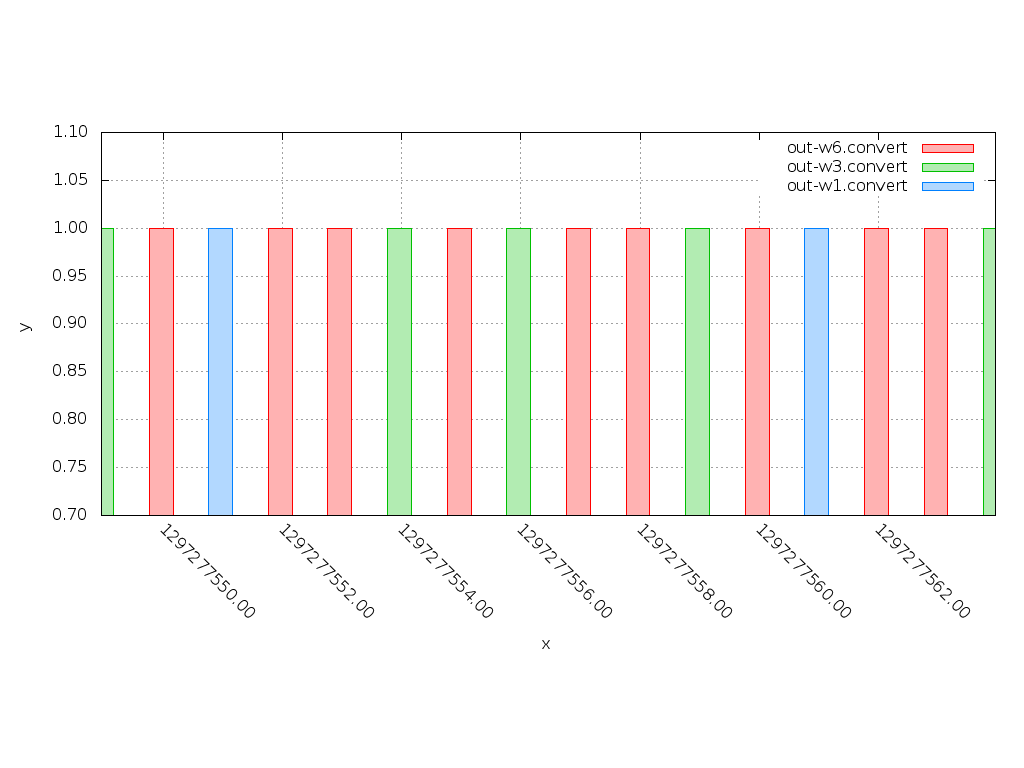
\includegraphics[width=0.70\textwidth]{wrr-dense.png}
	\captionof{figure}{Testing \texttt{WRRSched} element}
	\label{fig:test-wrr}
  \end{center}

  \subsection{Weighted Deficit Round Robin scheduler}
  Similar to Weighted Round Robin (WRR), we also have two versions for Weighted Deficit Round Robin scheduler: compound element and new element.
  \subsubsection{WDRR scheduler - compound element}
  \textbf{Location:} \texttt{4-scheduler/WDRR\_Sched.click}.\\
  The way of implementation is the same as WRR scheduler (compound element), that is to provide more input ports of Deficit Round Robin scheduler to the high weight input flows. Figure \ref{fig:test-wdrr-compound} shows the distribution of packets of each flow on the output link. We setup three flows with packet length 500, 1000, 1500 byte, and weights 1, 2, 3 respectively. We can see that a number of packets of each flows is nearly the same as we expect.
  \begin{center}
	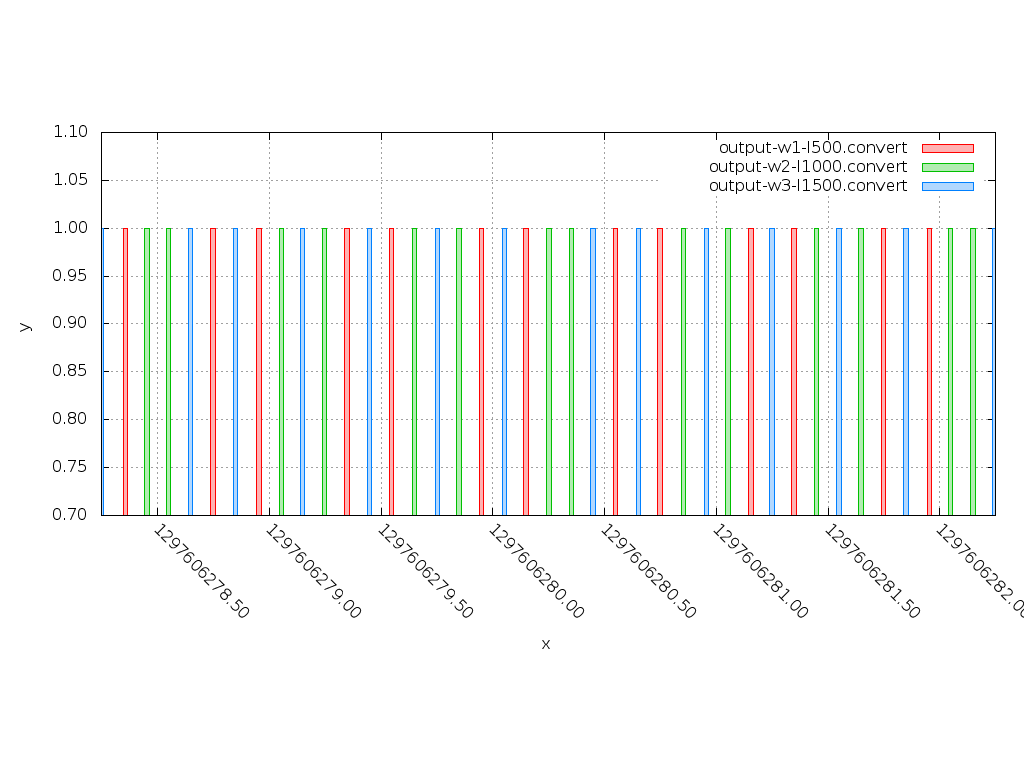
\includegraphics[width=0.70\textwidth]{wdrr-dense-compound.png}
	\captionof{figure}{Testing \texttt{WDRRSched} compound element}
	\label{fig:test-wdrr-compound}
  \end{center}

  \subsubsection{WDRR scheduler - new element}
  \textbf{Location}: \\
  \texttt{elements/wdrr.\{cc,hh\}} \\ 
  \texttt{4-scheduler/WDRR\_Sched\_element.click}\\
  There are some problems that motivate us to implement a new element for WDRR:
  \begin{itemize}
  	\item Quantum is fixed. It is not fair to flows having large size packets.
  	\item Weights cannot be positive real number.
  	\item Weights cannot be changed in runtime.
  \end{itemize}
  By inheriting from source code of DRR scheduler, we have just needed to modify at the time updating deficit: 
  \begin{align*}
    new\_deficit = old\_deficit + quantum * weight;
  \end{align*}
  We test this element with three flows. Flow0 has 100 byte of packet length, weight $0.2$. Flow1 has 200 byte of packet length, weight $0.4$. Flow2 has 400 byte of packet length, weight $0.8$. Output flow is shown in Figure \ref{fig:test-wdrr-element}. We can see that with these parameters, WDRR scheduler operates like a Round Robin scheduler.
  \begin{center}
	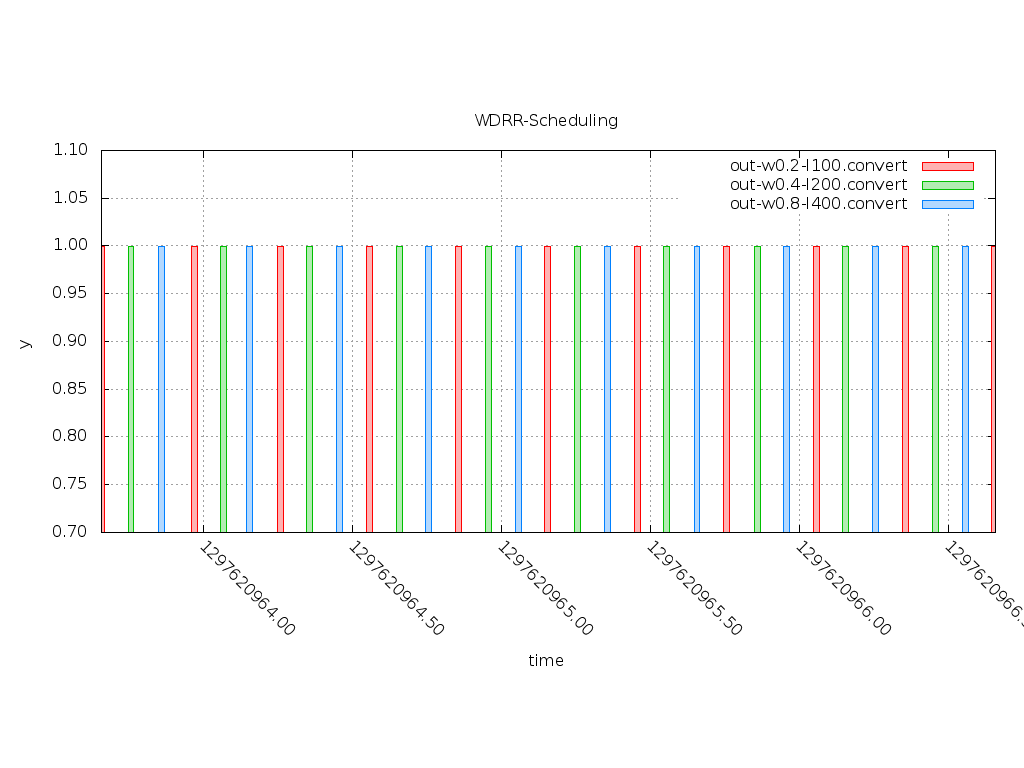
\includegraphics[width=0.70\textwidth]{wdrr-dense-element.png}
	\captionof{figure}{Testing \texttt{WDRRSched} element}
	\label{fig:test-wdrr-element}
  \end{center}
  
  Since this element allows real numeric weight, there are some applications of this element:
  \begin{itemize}
  	\item Round Robin scheduling (figure \ref{fig:test-wdrr-element}). For each flow, setup
  	\begin{align*}weight &= \frac{avg\_packet\_length}{quantum}\end{align*}
  	\item Round Robin scheduling with some burst duration. For each flow, setup 
  	\begin{align*}weight = \frac{burst\_duration*avg\_packet\_length}{quantum}\end{align*}
  	\item Give more fairness in response time. For example, assume there are two flows: packet length in flow 0 is 100 byte, and packet length in flow 1 is 200 byte. With the built-in DRR scheduler, the sequence of packets on the output link is:
  	  \begin{align*}f0, f0, f0, f0, f0, f1, f1, f0, f0, f0, f0, f0, f1, f1, f1, ... \end{align*}
  	where $f0$, $f1$ are represented to a packet from flow0 and flow1 respectively. We can do more better by using WDRR scheduler with weights 0.2, 0.2. The sequence of packets is changed as:
  	  \begin{align*}f0, f0, f1, f0, f0, f1, f0, f0, f1, f0, f0, f1, f0, f0, f1, ... \end{align*}  	 
  \end{itemize}
  
  \subsection{\texttt{SetVirtualClock} element} \label{section:virtualclock}
  \textbf{Location}: \texttt{elements/setvirtualclock.\{cc,hh\}}\\
  It is a new Click element which is used to support Virtual Clock scheduler and Weighted Fair Queue scheduler. Its important feature is the ability of remembering the last computed values (virtual time, tag). Each time a packet arrives, it will set a new tag into timestamp annotation of packet. Computation of tag and virtual time is based on these equations: \\ 
  \begin{align*}
  F_{i}^{k} &= \max(F_{i}^{k-1}, V(a_{i}^{k})) + \frac{L_{i}^{k}}{r_i}\\
  V(0) &= 0 \\
  \frac{\partial V}{\partial \tau} &= \frac{1}{\sum r_j} \\
  \end{align*}
  To use this element, user needs to provide: $rate$ (bandwidth of a flow), $max\_bw$ (maximum bandwidth of output link), $current\_bw$ (current used bandwidth of output link). At runtime, this element allows user to read $last\_tag$ and also modify $rate$, $max\_bw$, $current\_bw$. When a packet arrives to this element, it does the following tasks:
  \begin{itemize}
  	\item Update virtual time: 
  	\begin{align*}last\_virtual\_time += \frac{(current\_real\_time - last\_real\_time)*max\_bw}{current\_bw}\end{align*}
  	\item Update tag:
  	\begin{align*}last\_tag = \max(last\_tag, last\_virtual\_time) + \frac{packet\_length}{rate}\end{align*}
  	\item Update packet's timestamp annotation to $last\_tag$
  	\item Update parameter of \texttt{SetVirtualClock}: $last\_real\_time$ to the current time.  	
  \end{itemize}
  Note: when configuring \texttt{SetVirtualClock} with $max\_bw = current\_bw$, the virtual time is exactly the real time. We can use this property to implement GCRA and Virtual Clock scheduling.
  \subsection{Virtual Clock scheduler}
  \textbf{Location}: \texttt{4-scheduler/VC\_Sched.click}\\
  We implement the Virtual clock scheduler with support of \texttt{SetVirtualClock}. Each flow is connected to a \texttt{SetVirtualClock} and then to a \texttt{TimeSortedSched} (Figure \ref{fig:vcsched}). Element \texttt{SetVirtualClock} is set up with $MAXBW = CURRENTBW$.  

  \begin{center}
	\includegraphics[width=0.80\textwidth]{test-vcsched.pdf}
	\captionof{figure}{\texttt{VirtualClock} scheduler with 3 flows}
	\label{fig:vcsched}
  \end{center}
  Scenario of testing Virtual Clock scheduling: There are three flows,
  \begin{itemize}
  	\item Flow 0: Rated source, packet length 1 byte, rate 1 pps.
  	\item Flow 1: Rated source, packet length 1 byte, rate 1 pps.
  	\item Flow 2: Rated source, packet length 1 byte, rate 3 pps.
  \end{itemize}
  We set up three \texttt{SetVirtualClock} with the same parameters: 
  \begin{align*}RATE = 1, MAXBW = 3, CURRENTBW = 3\end{align*} 
  These parameters said that each flow can only use one-third bandwidth of output link. Output link speed is 1pps. Flow 2 is postponed 5 second later than flow 0 and flow 1. The result is shown in figure \ref{fig:test-vcs1}. We can see that when flow 2 starts to send packets, it does not make large effect to other flows but shares the output with others.
  
  \begin{center}
	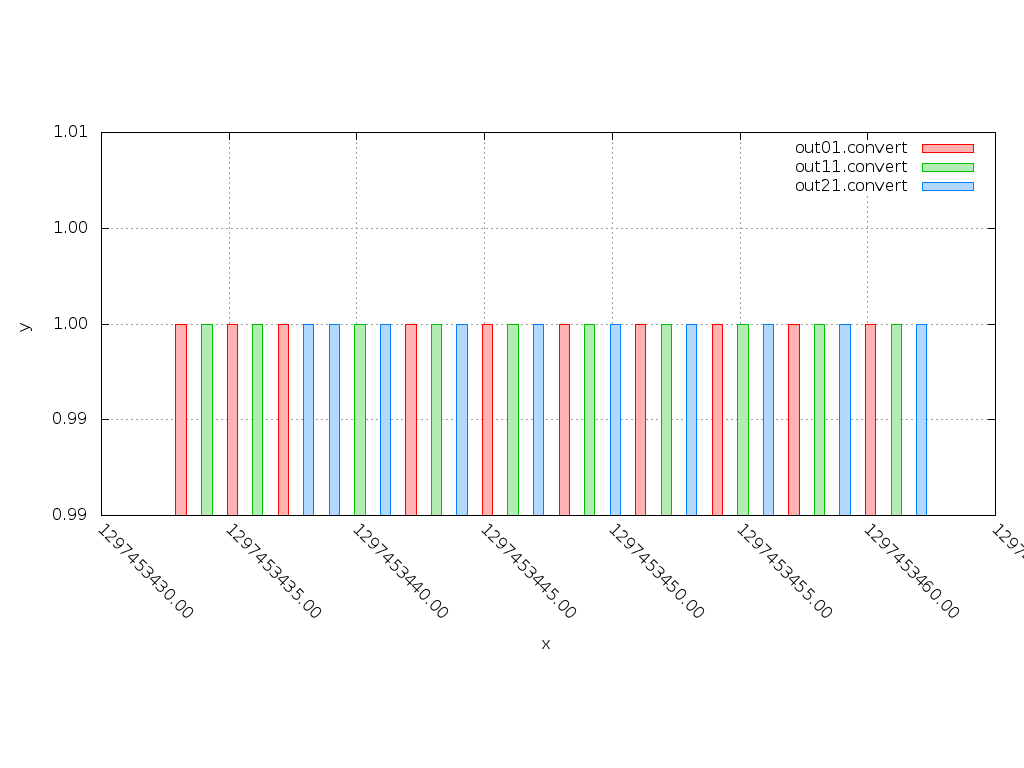
\includegraphics[width=0.80\textwidth]{vcs1-dense.png}
	\captionof{figure}{Testing \texttt{VirtualClock} scheduler with 3 flows}
	\label{fig:test-vcs1}
  \end{center}
  
  %\subsection{Weighted Fair Queue scheduler}
  \section{Congestion control}
  \subsection{Weighted RED buffer management}
  We want to build a Weighted RED (WRED) based on RED element. A WRED allows us to define some ranges of bandwidth, each range has a particular probability of dropping packets. The idea of implementation: Packets are classified by their rate (or a range of rate), and then let them go through a RED element used for this rate. We check this idea by writing a WRED that support two ranges of rate, see figure \ref{fig:wred2}.
    \begin{center}
	  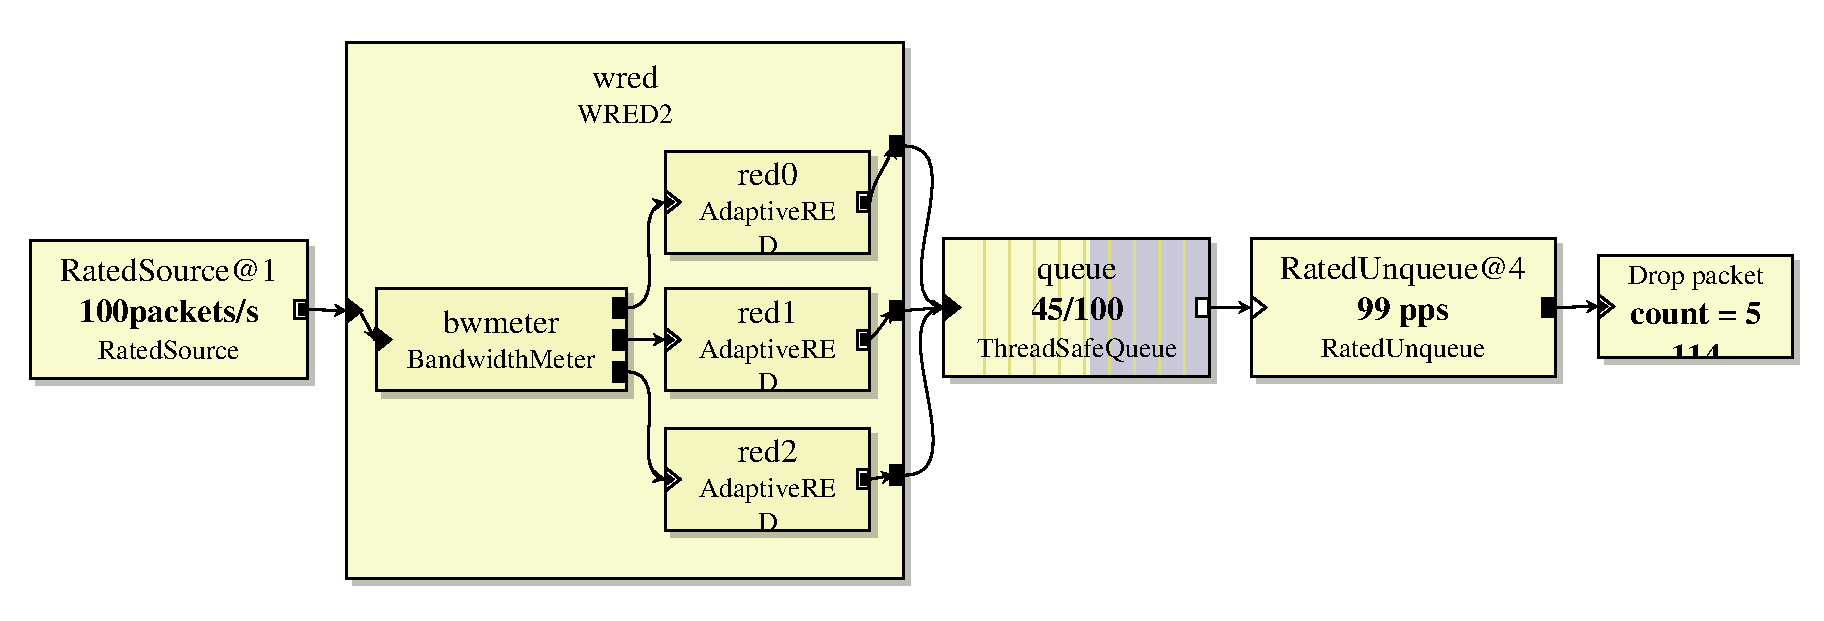
\includegraphics[scale=0.5]{wred2.pdf}
	  \captionof{figure}{One simple implementation of \texttt{WRED} element}
	  \label{fig:wred2}
    \end{center}
  
\end{document}
